%-------------------------------------------------------------------------------
% IPOL LaTeX class manual
% by rafael grompone von gioi
% ver 0.5 - July 1, 2014
%-------------------------------------------------------------------------------
\documentclass{ipol}
\usepackage{mathrsfs} 
\usepackage{xfrac}
\usepackage{amsmath} 
\usepackage{amsfonts}
\usepackage{rotating} 
\usepackage{fancyvrb} 
%%for subfigure using ?
\usepackage{graphicx}
\usepackage{caption}
\usepackage{subcaption}
\usepackage{makeidx}
\usepackage{authblk}
\usepackage{algorithm}
\usepackage{algorithmic}  
\usepackage{amsthm}
\usepackage[normalem]{ulem}
%\usepackage{subfigure}

\ipolSetTitle{Epipolar rectification of a generic camera}
\ipolSetAuthors{Marc Pierrot Deseilligny\ipolAuthorMark{1},
                Ewelina Rupnik\ipolAuthorMark{1}}
\ipolSetAffiliations{%
\ipolAuthorMark{1} LASTIG, Univ Gustave Eiffel, ENSG, IGN, F-94160 Saint-Mande, France\\
                   (\texttt{marc.pierrot-deseilligny@ensg.eu}, \texttt{ewelina.rupnik@ign.fr})
%\\\ipolAuthorMark{2} IIE, UdelaR, Uruguay (\texttt{jirafa@fing.edu.uy})
}

%---------------------------------------------
\newcommand{\CPP}{\mbox{\tt C\hspace{-0.05cm}\raisebox{0.2ex}{\small ++} }}
\newcommand{\SiftPP}{\mbox{\tt Sift\hspace{-0.05cm}\raisebox{0.2ex}{\small ++} }}



\newcommand{\RR}{\ensuremath{\mathbb{R}}}
\newcommand{\COM}[1]{}
\newcommand{\LA}{ LLLLLLLLLLLLLLLLLLLLLLLLLLLLLLLLLLLLLLLLLLLLLLLLLLLLLL \\ \\ }
\newcommand{\LALA}{ \LA \LA \LA \LA \LA \LA \LA \LA \LA \LA \LA \LA \LA \LA \LA  }


%// \newcommand{\HComp}{{}^{\longleftrightarrow}_{\pi_1,\pi_2}}
\newcommand{\HComp}{\overset{\Longleftrightarrow}{\scriptscriptstyle \pi_1,\pi_2}}
\newcommand{\PiOT}[1]{\pi_1(\pi_2^{-1}(#1))}
\newcommand{\PiTO}[1]{\pi_2(\pi_1^{-1}(#1))}
\newcommand{\CurvO}{{\mathcal{T}_1}}

%  Bundles
\newcommand{\Bund}[1]{\ensuremath{\mathcal{B}_{#1}}}
\newcommand{\BundO}{\Bund{1}}
\newcommand{\BundT}{\Bund{2}}
\newcommand{\BundK}{\Bund{k}}


% Epipolar lines
\newcommand{\LineE}[1]{\ensuremath{\mathcal{L}_{#1}}}
\newcommand{\LineO}{\LineE{1}}
\newcommand{\LineT}{\LineE{2}}
\newcommand{\LineK}{\LineE{k}}

\newcommand{\CurveE}[1]{\ensuremath{\mathcal{C}_{#1}}}
\newcommand{\CurveO}{\CurveE{1}}
\newcommand{\CurveT}{\CurveE{2}}
\newcommand{\CurveK}{\CurveE{k}}

% "Epipolar Surface"
\newcommand{\Sv}{\ensuremath{\mathcal{S}_{v}}}

\newcommand{\BigV}[1]{\ensuremath{\overrightarrow{#1}}}
\newcommand{\TanO}[1]{\BigV{t_1#1}}
\newcommand{\TanT}[1]{\BigV{t_2#1}}

\newcommand{\Negl}[1]{\ensuremath{\mathcal{O}(#1)}}



\newcommand{\PiVert}{\widetilde{\pi}}
\newcommand{\PiZVert}{\widetilde{\pi}_1^{\mathcal{Z}} }
%\newcommand{\PiOT}{\Pi^{12}}
%\newcommand{\PiTO}{\Pi_{2\rightarrow 1}}

\newcommand{\DerPart}[2]{\frac{\partial #1}{\partial #2}}

\newtheorem{theorem}{Theorem}
\newtheorem{notation}{Notation}
\newtheorem{definition}{Definition}
\newtheorem{remark}{Remark}

\definecolor{orange}{rgb}{1,0.5,0} 
\newcommand{\er}[1]{\textcolor{orange}{#1}} 
\definecolor{magenta}{rgb}{1,0,1} 
\newcommand{\mpd}[1]{\textcolor{magenta}{#1}} 
\newcommand{\ChangeMPD}[2]{\textcolor{blue}{#2}} 

\definecolor{blue}{rgb}{0,0,1} 
\newcommand{\ermpdok}[1]{{\bf \textcolor{blue}{#1}} }

\definecolor{black}{rgb}{0,0,0} 
\newcommand{\BEGINCHANGE} {\textcolor{magenta}{ ---------------------------------------BEGIN-BEGIN-BEGIN}}
\newcommand{\ENDCHANGE}{\textcolor{magenta} {END-END-END------------------------------------------------}}


%-------------------------------------------------------------------------------
\begin{document}

%-------------------------------------------------------------------------------
\begin{ipolAbstract}
We propose a generic method for epipolar resampling that is not tied to a specific camera model. We demonstrate the effectiveness of the approach on a central perspective, pushbroom and pushbroom panoramic camera models. We also devise an \textit{epipolarability index} that measures the suitability of an image pair for epipolar rectification, and provide a formal derivation of the ambiguity bound to epipolar resampling. 
\end{ipolAbstract}

%-------------------------------------------------------------------------------
\ipolKeywords{epipolar rectification, generic camera, pushbroom sensor, central perspective}

%-------------------------------------------------------------------------------


\section{Introduction}
The epipolar geometry of images plays a central role in many applications in the field of photogrammetry and computer vision. In the stereo-reconstruction pipeline, it is used twice:

\begin{enumerate}
   \item In the camera pose orientation step, when computing the
      relative orientation of a pair of images from their corresponding points. Assuming 
      the projection follows the central perspective and the internal calibration is known,
      one can compute the epipolar geometry of the images using the essential matrix. Finally, the relative orientation is recovered \cite{fusiello2000epi}.   
     
   \item In the image dense matching step, where the epipolar rectification simplifies the 
       correspondence search because for any point $(x_1,y)$ in image $I_1$, its correspondence is some point $(x_2,y)$ in image $I_2$. Therefore, finding correspondences across images is reduced to 
        a $1$-dimensional problem ($1$D).
\end{enumerate}

\noindent In this paper, we only look at the epipolar rectification problem and more specifically
its application to a generic camera model.%, focusing on the pushbroom sensors.

\subsection{Related works}
Rectifying a central perspective camera stereo pair involves transforming their original epipolar geometry to a canonical form where: (a) their focal planes are coplanar, and (b) their conjugate epipolar lines are colinear, and parallel to the camera's x-axis. 
%It is equivalent of sending the stereo pair's epipoles at infinity. 
From the algebraic standpoint, this is equivalent to applying two $2$-dimensional ($2$D) projective transformations to both images of the stereo pair. Several approaches to computing such transformations have been proposed over the course of the last 30 years.

For a calibrated stereo pair (i.e. with known camera projection matrices), there exists a unique rectifying transformation, up to a rotation along the baseline~\cite{fusiello2000epi}. In an uncalibrated case, the solution is obtained by factoring out two 2D homographies from the fundamental matrix. Because there are no two unique homographies, the common practice is to parametrize these transformations such that the distortions caused by the rectification process are minimized. For instance, Loop and Zhang~\cite{loop1999epi} decompose the rectifying homographies to a combination of the projective, similarity and shearing transforms, with the condition that the prrojective transform remains (close to) affine. Hartley~\cite{hartley1999epi} satisfies the condition that for a neighborhood of a point (e.g. the center of an image), the computed homography is a rigid transformation. Building on this work, Isgro and Trucco's~\cite{isgro1999epi} approach obtains a unique solution by minimizing the x-disparity without having to explicitly calculate the fundamental matrix. Instead of minimizing the disparity in the first coordinate, Wu and Yu~\cite{wu2005epi} recycle an idea first introduced by Hartley~\cite{hartley1999epi} which requires that the aspect ratio of the images before and after rectification is constant. More recently, Fusiello and Irsara~\cite{fusiello2008epi} introduced the camera matrices back into the equation and proposed a \textit{quasi}-Euclidean approach for uncalibrated cameras, similar to that of the calibrated cameras case. Their projective transformations are parametrized by five angles and a focal length. Monasse \textit{et al.}~\cite{monasse2010epi} break down the one-time rotation of~\cite{fusiello2008epi} to a three step procedure, and prove increased robustness by using a geometric error measure (i.e., camera rotation angle) to reduce the rectifying error distortions.

%force the plane at infinity to be close to the plane at infinity of a calibrated stereo pair. This is possible by making an educated guess and estimating only the focal length.


 
%Epipolar recitification algorithms for central projection cameras can be classified into calibrated and uncalibrated camera approches.


%For central projection cameras, the epipolar recitification algorithms are grouped into the calibrated and uncalibrated camera case. Rectifying calibrated cameras comes down to fixing their perspective center and rotating the cameras until their focal planes are coplanar (Fusiello compact algo). Uncalibrated camera rectification involve additional parameters 

  
%
Unlike the central projection camera model, pushbroom-like sensors acquire each image row from a different perspective center. As a consequence, the epipolar lines are neither straight lines, nor are they conjugate across the image~\cite{Gupta1997}.  One way to overcome this particularity is to simplify the projection function with a 2D affine~\cite{ono1999epipolar,wang2011epipolar} or a parallel projection model~\cite{morgan2006epipolar}. Such approximations usually come at the price of precision, especially with the increasing camera field-of-view or in mountainous scenes. By extending the 2D affine model with two quaratic terms, Okamonoto \textit{et al.}~\cite{okamoto:99:DLT} demonstrates improved performance on SPOT images. In the context of dense image matching, de~Francis \textit{et al.}~\cite{deFrancis2014stereo} improves the precision by partitioning the images into small patches, for which indepedent affine rectifictions are computed. Alternatively, and with equally good precision, Oh~\cite{Oh2011} uses the \textit{Rational Polynomial Coefficients} (RPCs) to map the epipolar curves across the full size images with lines, in a piecewise approach, followed by a global rectification transformation using a polynomial function of 3$^{rd}$ order.
%
%ù while being locally approximated to straight lines. Oh~\cite{Oh2011} approximates the epipolar curves of an image pair by piecewise linear curves with a set of virtual correspondences. An image pair is then resampled to an equivalent geometry, imposing that the conjugate curves become straight and aligned on the y-axis. 


%uses the \textit{Rational polynomial coefficients} (RPCs) to trace the epipolar curves across image pairs with a dense set of virtual correspondences, and by doing so approximates the curves by a piecewise linear curve. Given a set of correspondences, an image pair is then resampled to an equivalent geometry, imposing that the conjugate curves become straight and aligned on the y-axis. 

%This work is similar to the approch proposed by Oh~\cite{Oh2011} in that it tries to model the epipolar curves across the entire image at once.
 
%  \cite{wang2011epipolar}

%The x-parallax remains linearly proportional to the depth of corresponding points - yes because we don(t move the x-coordinates

 
%\cite{orfeo2008}

%Carlo de Franchis , split the images in small patch, in each patch compute a coniq camera that approximate the model for each pair, make an epipolar resampling of this approximate coniq camera.  Advantage : simple an reuse existing method. Drawback : need small patch to be accurate enough.

\subsection{Contributions}
Our research work proposes an epipolar geometry rectification method that is not tied to any camera physical model. %Thus, our method can be applied to images taken with the central projection camera model and the pushbroom sensor. 
We provide a theoretical derivation and demonstrate the effectiveness of the approach on a range of models, including Pleiades images (pushbroom), the Corona images (panoramic pushbroom) and a consumer grade camera images (central perspective).
The method resembles Oh's~\cite{Oh2011} approach in that it exploits the point correspondences to find the polynomial mapping to epipolar geometry. However, unlike the work of Oh~\cite{Oh2011}, we do not require that the camera geometric model is known. We demonstrate that in some circumstances, point correspondences obtained from an image processing routine, e.g. SIFT~\cite{lowe2004distinctive}, can serve to find the epipolar resampling. 
Finally, we formally derive the ambiguity of the epipolar geometry, and propose an \textit{epipolarability index} that quantitatively describes the existence of epipolar geometry between a pair of images.

In the remainder of this publication, we first outlay the mathematical background of the epipolar geometry{, identify conditions required for its existence and establish its degree of ambiguity}  (Section~\ref{sec:math}). Then, we introduce our method (Section~\ref{sec:method}), and conclude with experiments on different datasets, with and without the geometric model (Section~\ref{sec:experiments}). 
 
\section{The mathematics of epipolar geometry in the generic case}\label{sec:math}

\subsection{Formalisation and notation of projections}

\begin{figure}[htb]
\centering
\begin{tabular}{c}
% \hline 
 \\
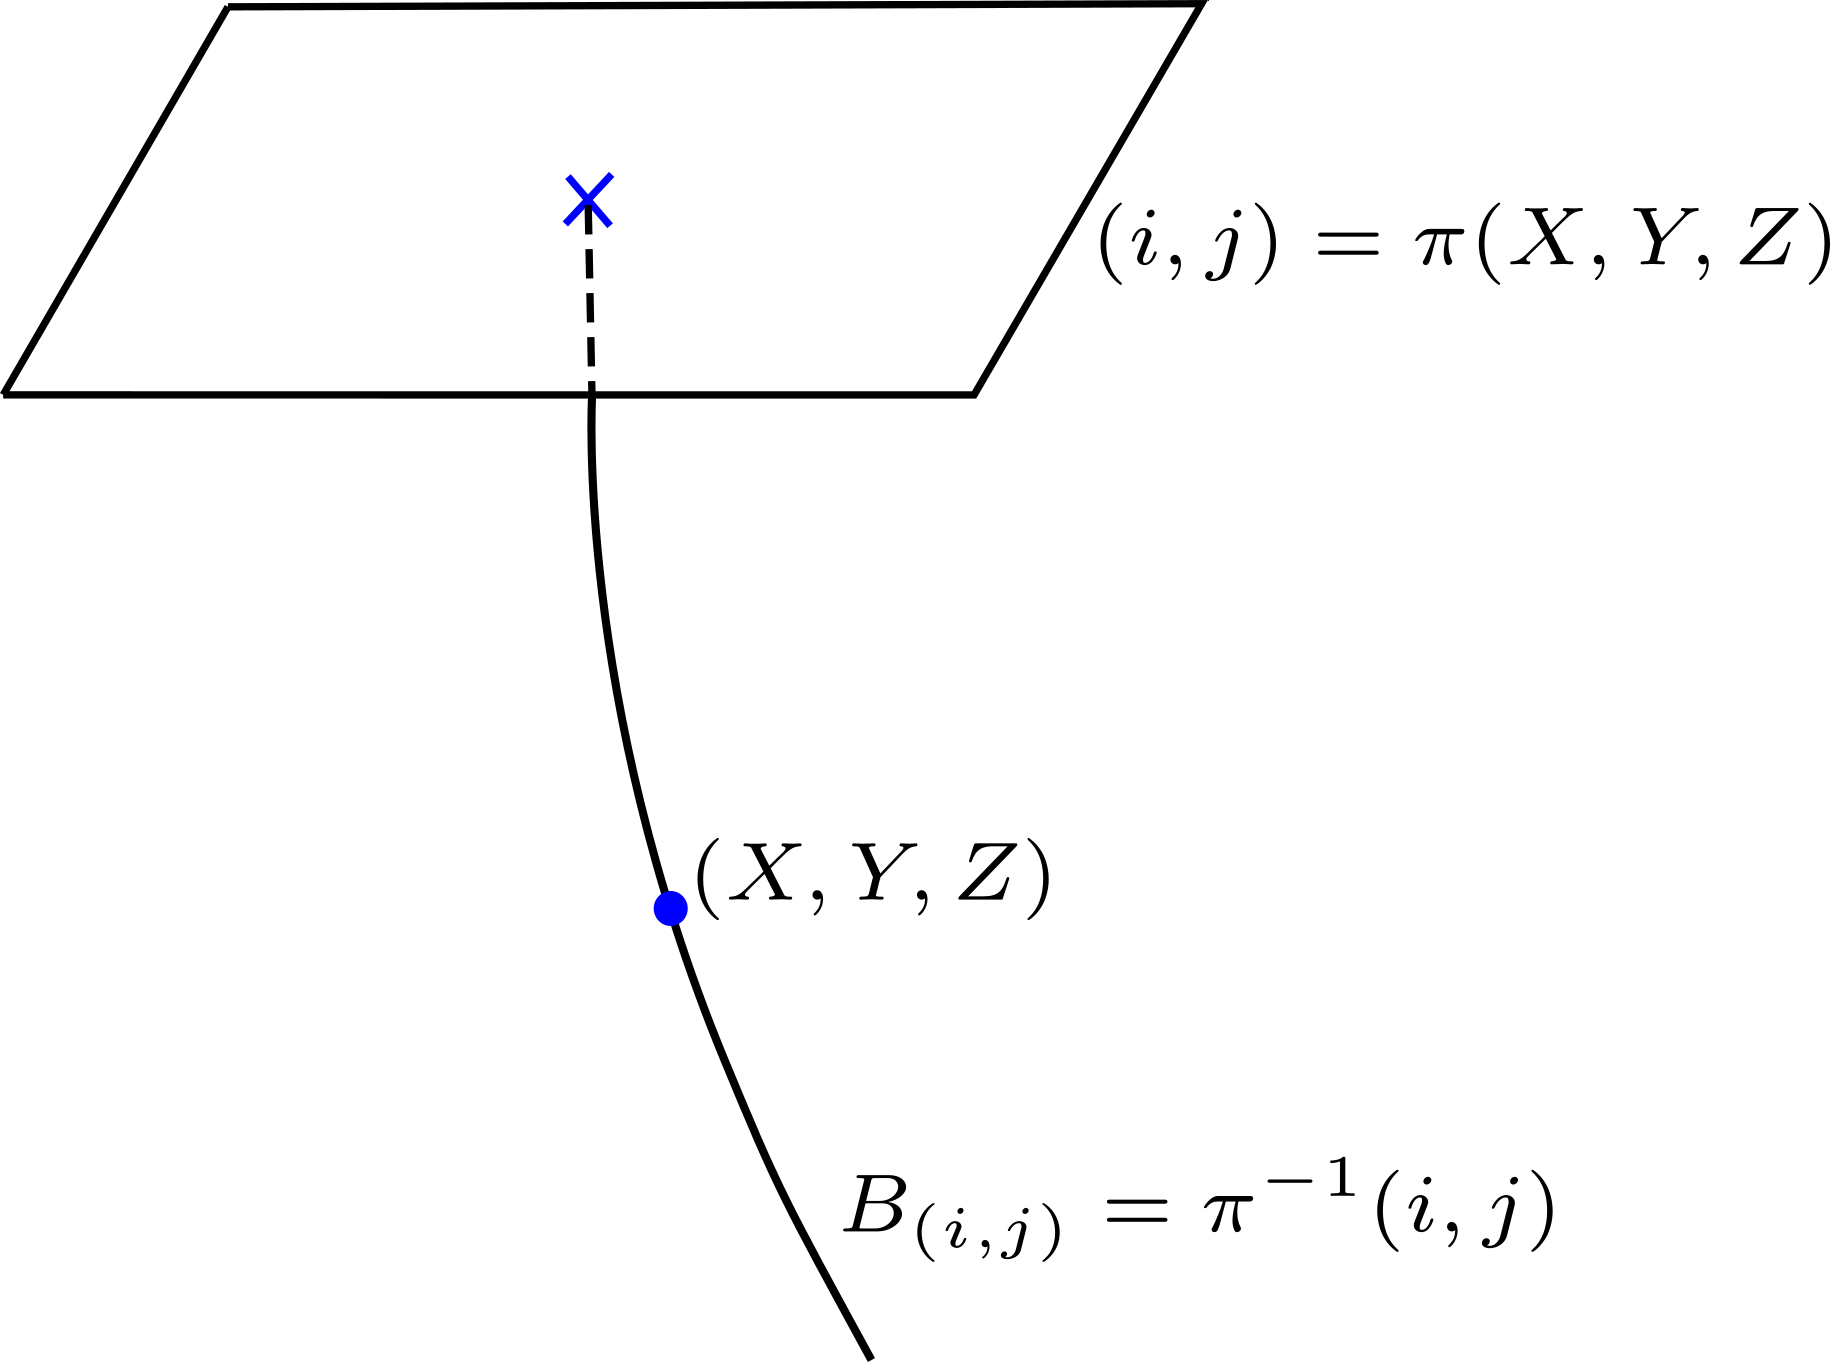
\includegraphics[width=6cm]{FIGS/NotaProj.png} 
 \\ 
  \\%\hline 
\end{tabular}
\caption{A projection and a bundle.}
\label{FigNotaProj}
\end{figure}



%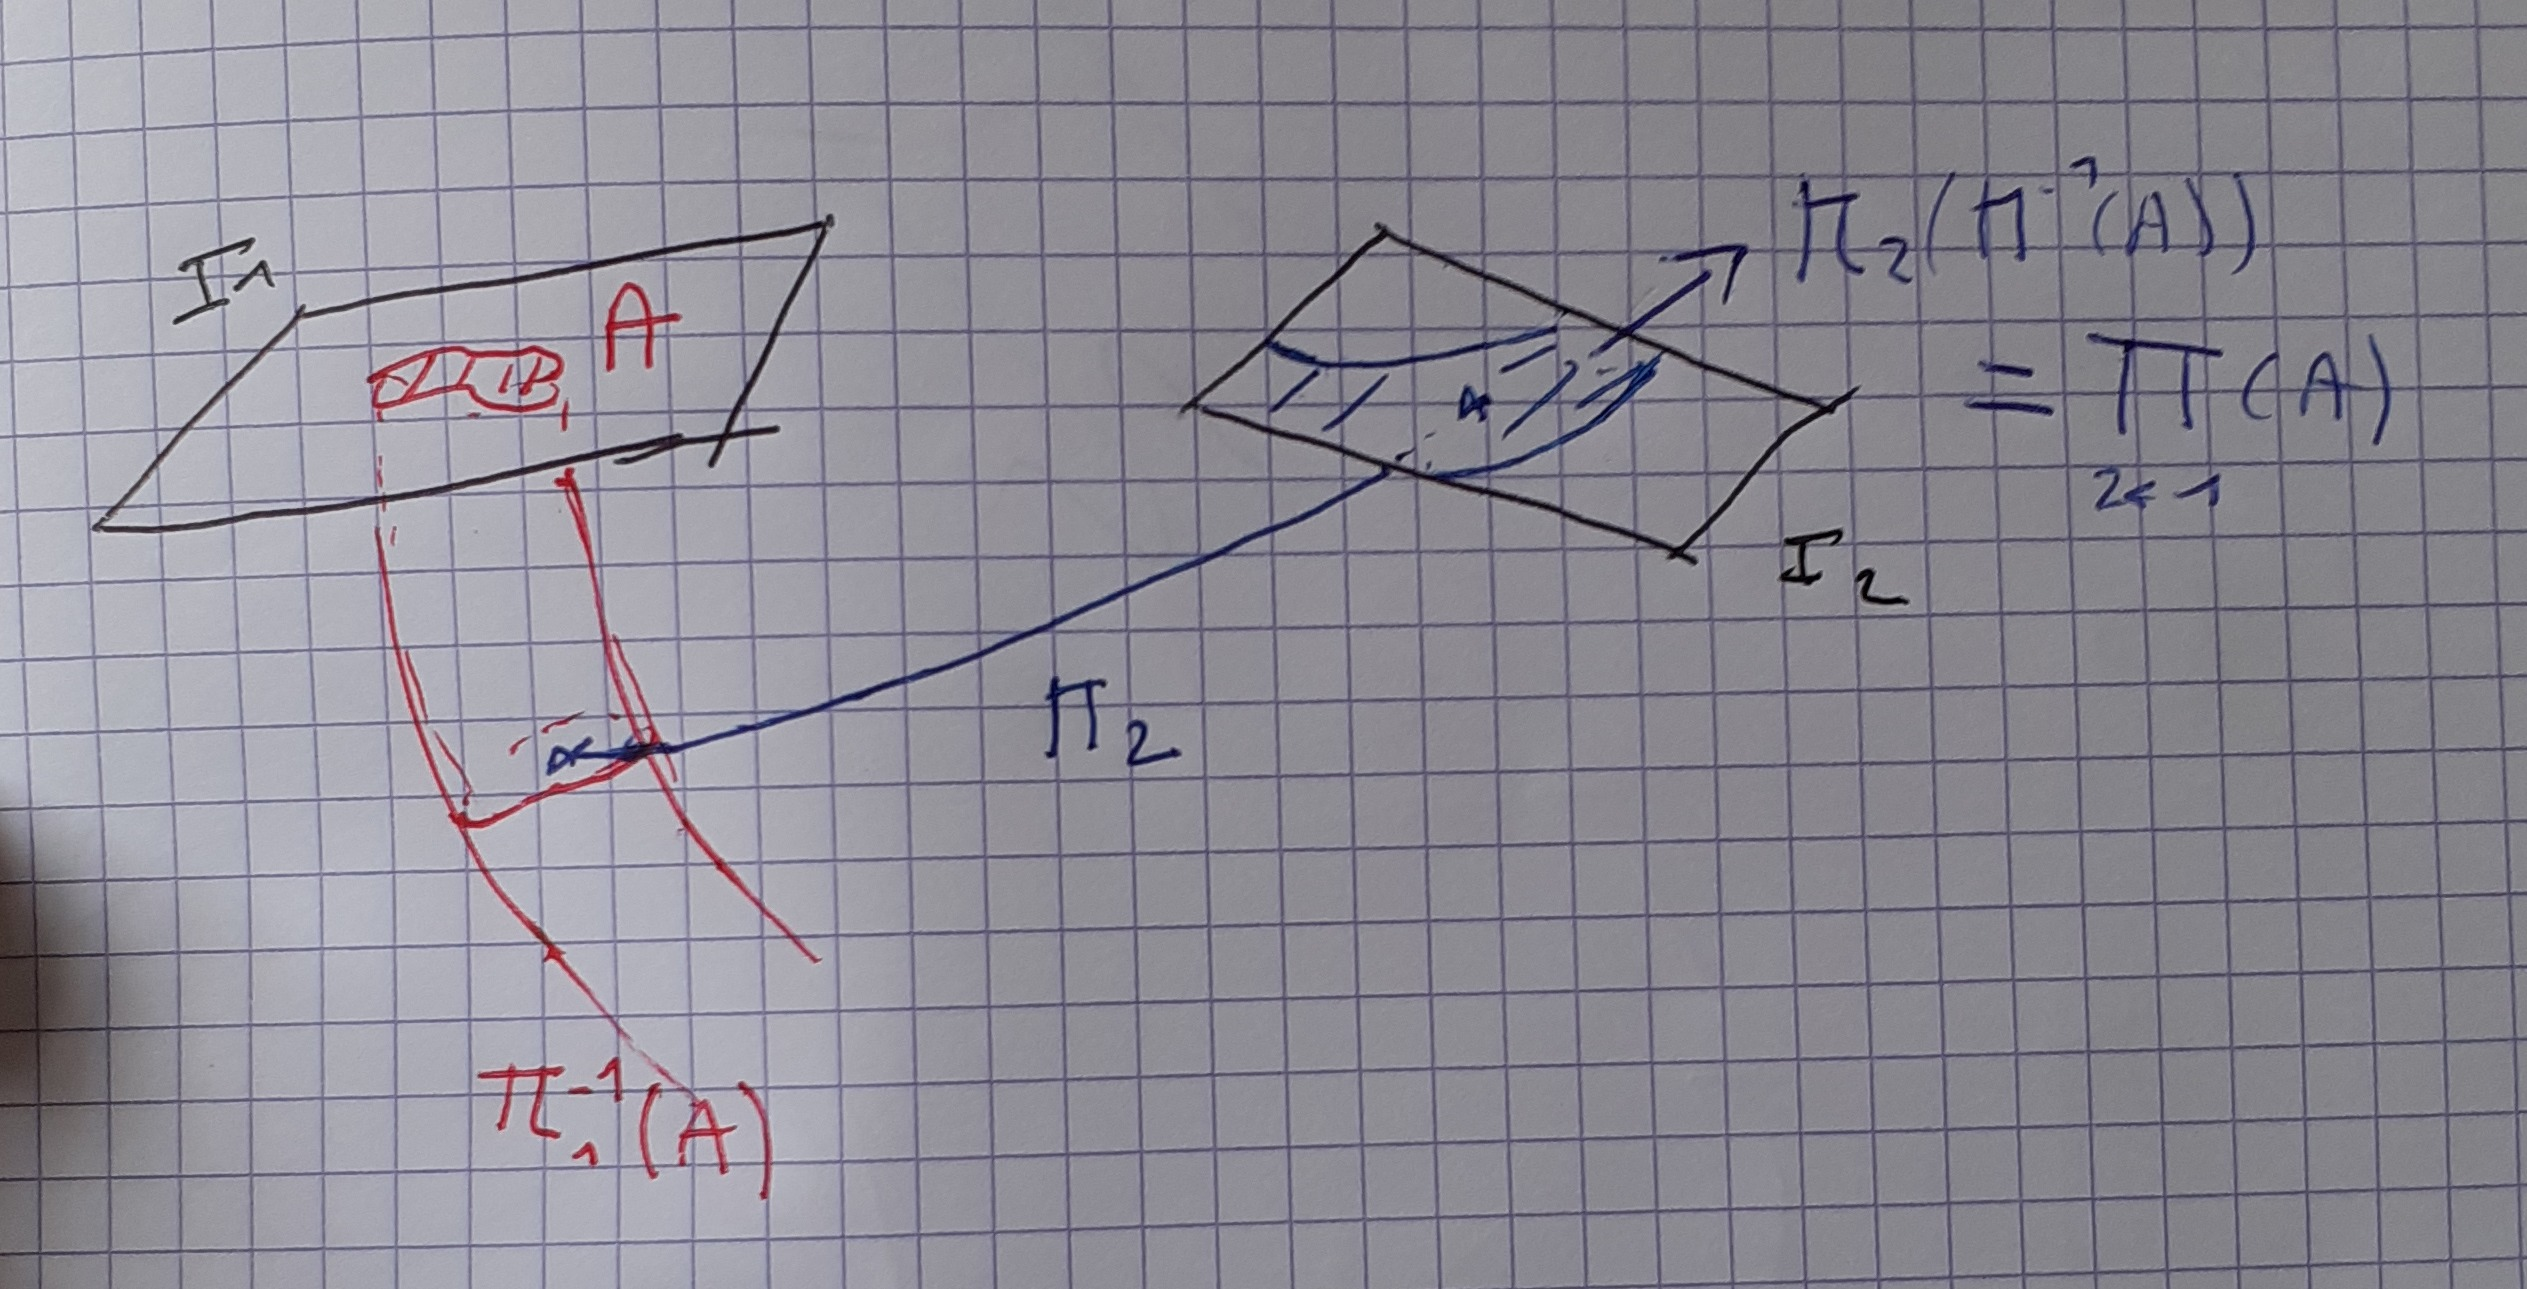
\includegraphics[width=12cm]{FIGS/NotaSets.jpg}

We define the geometric sensor model of an image by a projection function $\pi$, that computes, for a given 3D
point, its 2D projection in the image:

\begin{definition}[Generic geometric sensor model]  

\emph{Illustrated in Figure~\ref{FigNotaProj}.}

A geometric sensor model $\pi$ is a $\mathcal{C}^{\infty}$ mapping from ground space $(\RR^3)$ to image space $(\RR^2)$:

\begin{equation}
  \pi :  \RR^3  \rightarrow \RR^2  ,  (X,Y,Z)  \rightarrow (i,j) = \pi(X,Y,Z). \label{Eq:Proj}
\end{equation}
\end{definition}

\noindent Next, we define the bundles of a projection:

\begin{definition}[Bundle]
For $p_k \in I_k$ we note $\BundK(p_k)$  the bundle corresponding 
to $\pi_k^{-1}(p_k)$. When there is no ambiguity,
we note identically  $\BundK(P)$, where $P\in \RR^3$,
 the bundle corresponding to $\pi_k^{-1}(\pi_k(P)) = \BundK(\pi_k(P))$.
\end{definition}


\noindent Later, for simplicity, we will use the  {quasi-vertical} hypothesis, which allows us to extend $\pi$ to a
bijective mapping of $\RR^3$ and compute its inverse.

\begin{definition}[Quasi-vertical camera model]  
We say that the projection is quasi-vertical if the following mapping $\PiVert$ is a diffeomophism of $\RR^3$: \label{DefQuasiVert}
\begin{equation}
  \PiVert :  \RR^3  \rightarrow \RR^3  ,  (X,Y,Z)  \rightarrow (i,j,Z) = \PiVert(X,Y,Z)  , with (i,j) = \pi(X,Y,Z). \label{PiInvert}
\end{equation}
\end{definition}
%
Given $2$ images $I_1$ and $I_2$, the knowledge  of their geometric models $\pi_1$ and  $\pi_2$
reduces the matching between $2$ images to a 1D problem. In fact, given a point $p_1$ in $I_1$,
we can compute the 3D curve $\BundO(p_1)$ of  ground points that project to $p_1$ in $I_1$, and compute its
homologous curve in $I_2$ with $\pi_2(\BundO(p_1))$. We now define the H-compatible relation between two points
by the following definition:

\begin{definition}[H-Compatible, $\HComp$] 
\emph{Illustrated in Figure~\ref{FigNotaComp}.}

We say that $p_1$ in  $I_1$ and $p_2$ in $I_2$ are  $\pi_1-\pi_2$ H-compatible, and write $p_1 \HComp p_2$, if   the following condition is satisfied:

\begin{equation}
   ( \BundO(p_1) \cap  \BundT(p_2) \neq \emptyset    )
    \Leftrightarrow
  (\exists P \in  \RR^3 : \pi_1(P) =p_1 ,  \pi_2(P) = p_2).
\end{equation}
\end{definition}

\begin{figure}[htb!]
\centering
\begin{tabular}{c}
 %\hline \\
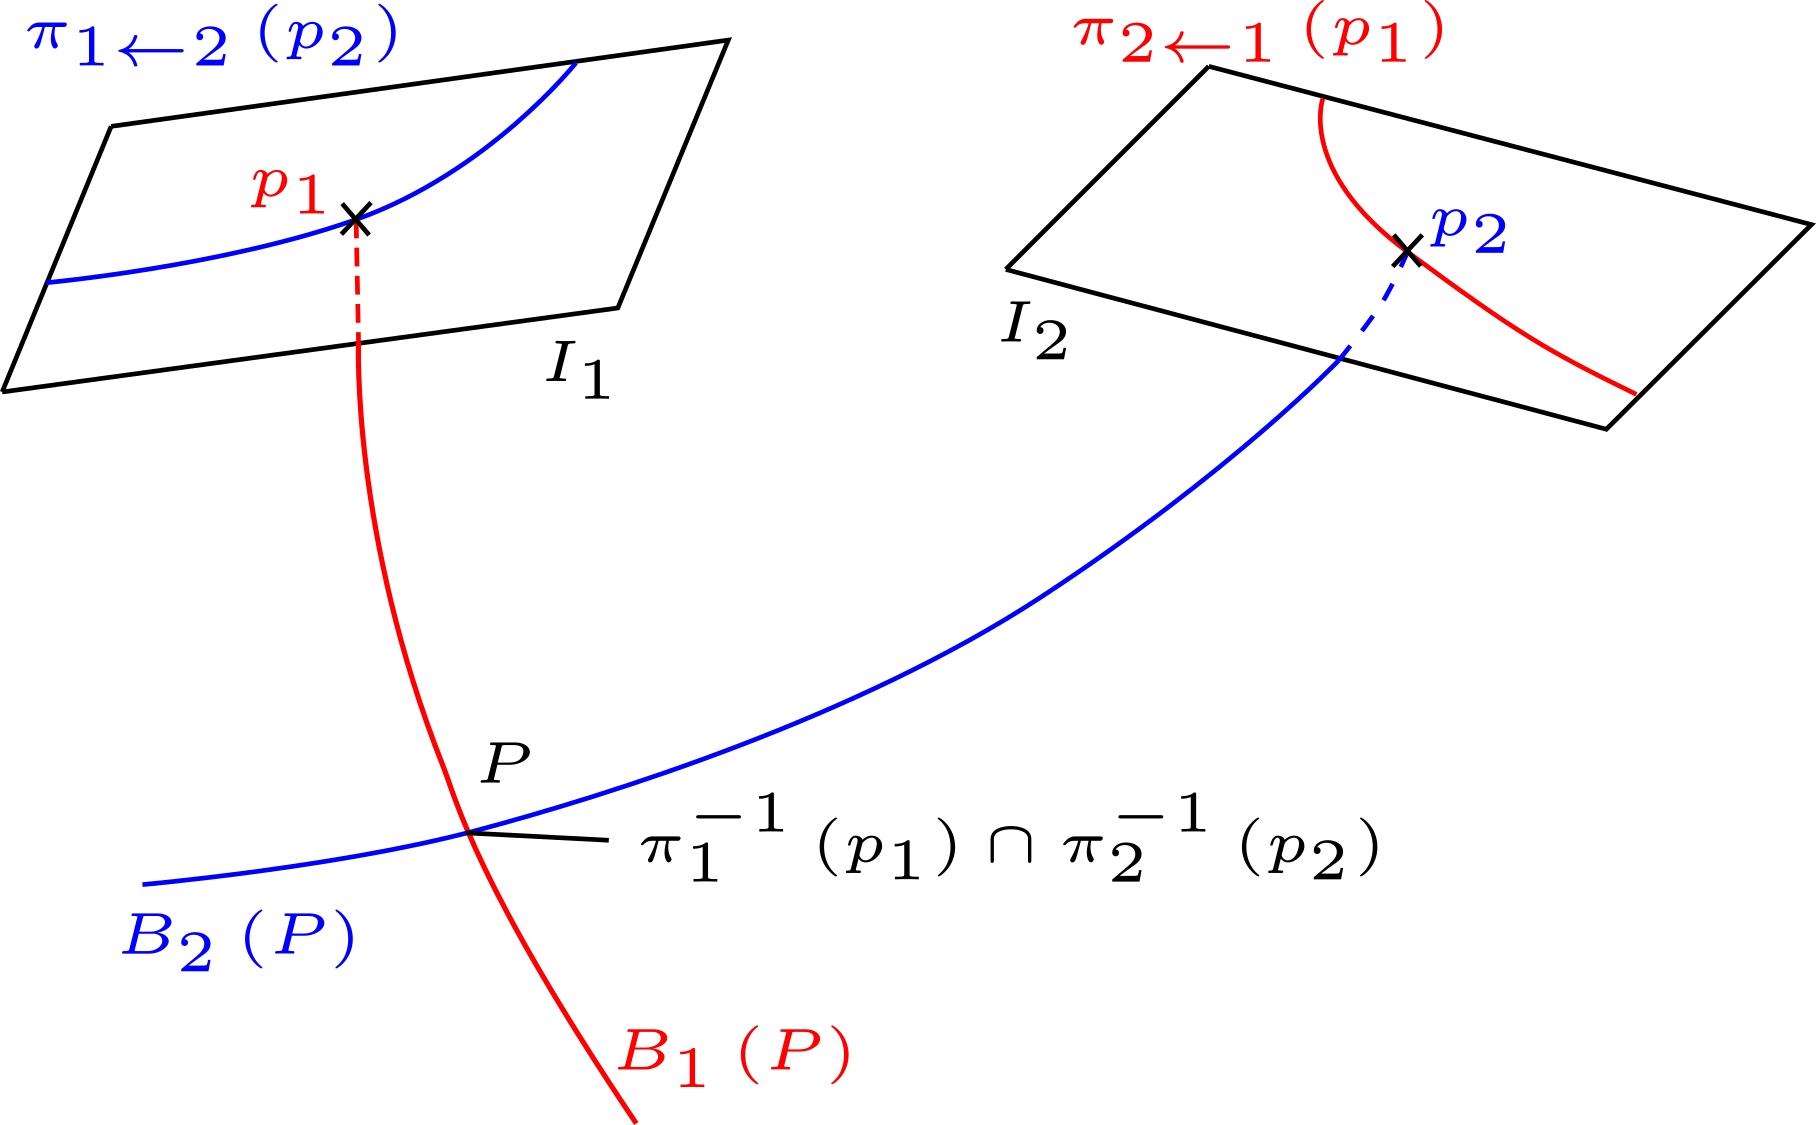
\includegraphics[width=9cm]{FIGS/NotaBundle.png} 
 %\\ \hline
\end{tabular}
\caption{Illustration of $\HComp$}
\label{FigNotaComp}
\end{figure}

\noindent In image matching, the relationship $p_1 \HComp p_2$  means that $p_1$ and $p_2$ are potentially homologous.

%---------------------------------------------
%---------------------------------------------
%---------------------------------------------



% - - - - - - - - - - - - - - -
\subsection{Definition of the epipolar geometry}

In fact, the previous relationships are sufficient to implement all the matching techniques and
$(\pi_1,\pi_2)$ can be used to define a matching process, taking advantage
of the~\emph{a priori} knowledge of the scene geometry. That is, given a point in one image, we can easily
follow its curve of potentially homologous points in the other image.
This technique, which does not exploit the epipolar geometry, has the advantage of also being adaptable to multi-image matching. Epipolar geometry is therefore not strictly required for the image matching process.

The drawback of this approach is that it combines two different problems in the same procedure: the handling of the geometry and resampling and
the matching process. When one is interested
in the matching of a single image pair, the epipolar geometry
can provide an elegant solution by separating the problem in two independent ones. 


\begin{definition}[Epipolar Geometry]
\emph{Illustrated in Figures~\ref{FigDefEpip} and~\ref{FigAmbigEpip}.}

Let $\pi_1,\pi_2$ be two cameras and let $\phi_1,\phi_2$  be two diffeomorphisms
of $\RR^2$. We say that $\phi_1,\phi_2$ are an epipolar resamplings iff:

\begin{equation}
  \forall e_1=(u_1,v_1) , e_2=(u_2,v_2) : (v_1=v_2)   \Leftrightarrow  (\phi_1^{-1}(e_1) \HComp \phi_2^{-1}(e_2)).
\end{equation}
   \label{EqEpiEgalY}
\end{definition}

\begin{figure}
\centering
\begin{tabular}{c}
 %\hline \\
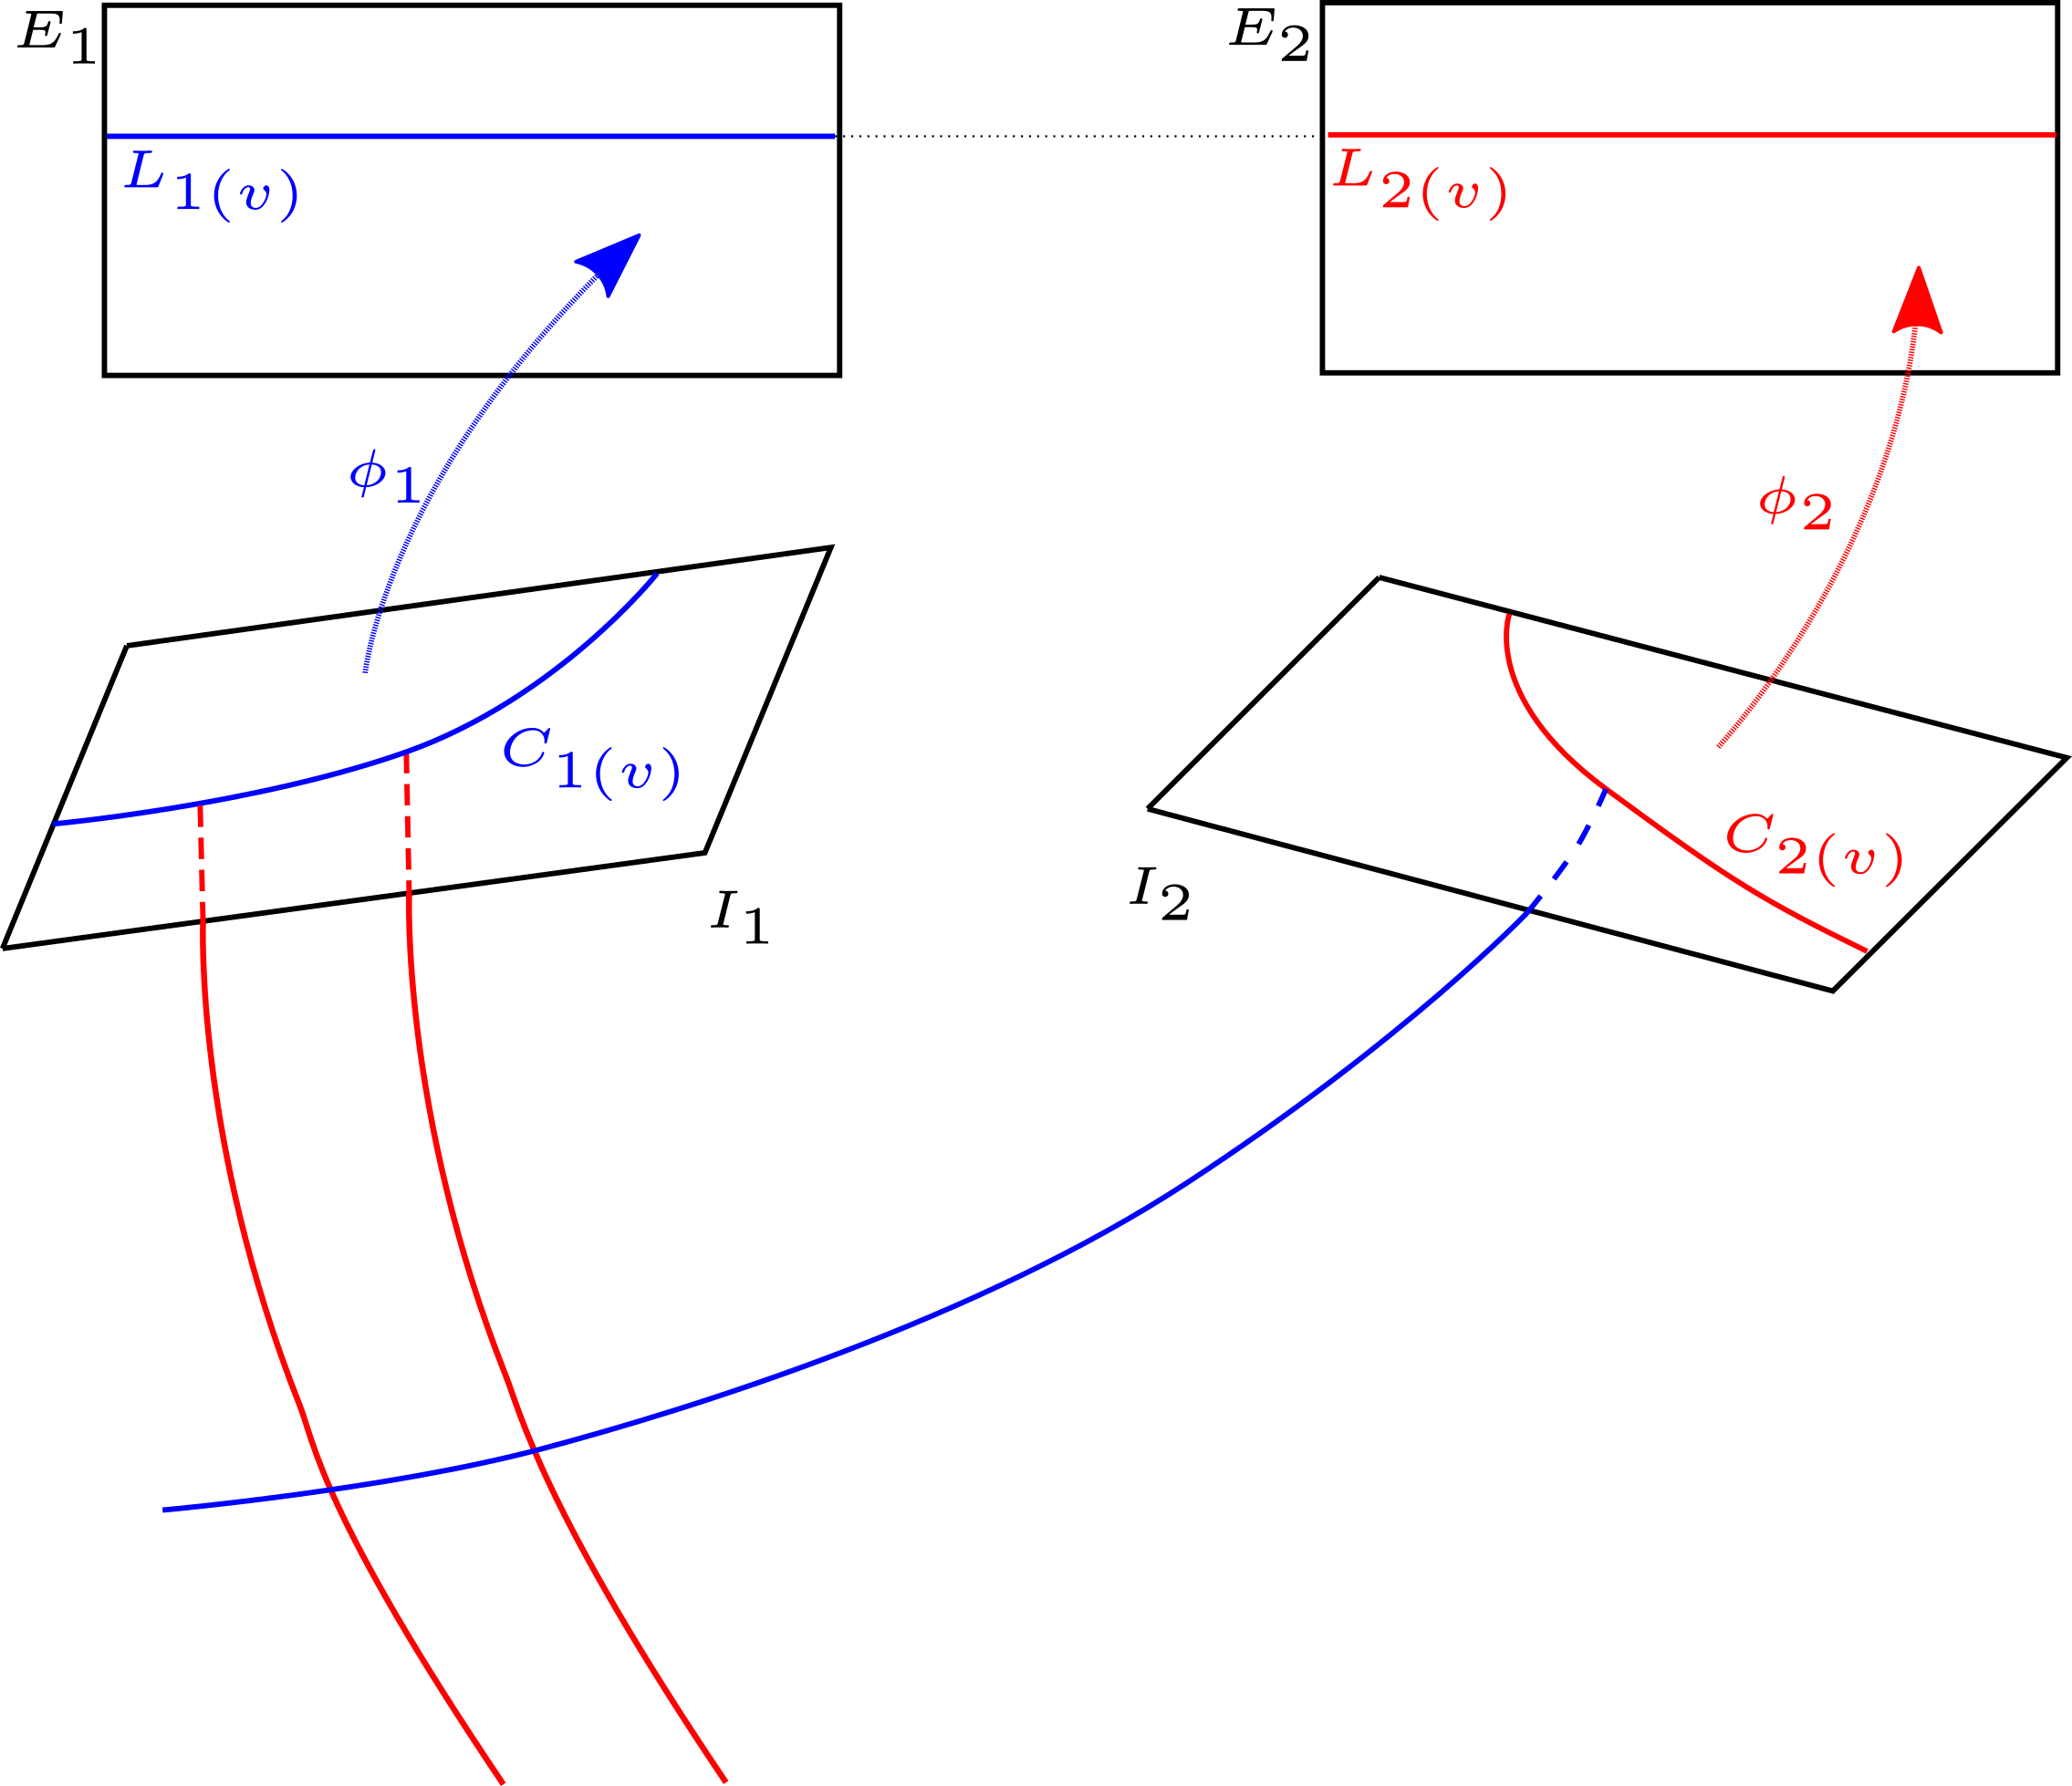
\includegraphics[width=9cm]{FIGS/Epip.png} 
 %\\ \hline 
\end{tabular}
\caption{Illustration of epipolar geometry.}
\label{FigDefEpip}
\end{figure}


\noindent The matching of epipolar images is simplified because we know that the lines in two images are globally homologous. 
%\er{The space of the image rectified to epipolar geometry is denoted by $E$ (see Figure~\ref{FigDefEpip})}


\begin{notation}[Epipolar line and curve.]
We denote $\LineK(v)$  as the epipolar  line of $E_k$ defined by $v_k=v$. We also denote $\CurveK(v)$ as the epipolar
curve of $I_k$ defined by $\CurveK(v) = \phi_k^{-1}(\LineK(v))$
\end{notation}
%
\noindent We can see that when epipolar geometry exists, the two curves $\CurveO(v)$ and $\CurveT(v)$ are globally homologous:

\begin{equation}
     \CurveO(v) = \PiOT{C_2(v)}   ;  \CurveT(v) = \PiTO{C_1(v)}.\label{Eq:CurvHom}
\end{equation}


%---------------------------------------------

%<<<<<<< HEAD
\subsection{Existence of the epipolar geometry}\label{ExistEpip} 

We now discuss the existence of the {epipolar geometry}. As it will be seen, the epipolar geometry generally does not exist, and when it does, it is not unique. We know that for any image pair following the {central projection}, there exists an epipolar geometry. However, with e.g. a cylindrical projection specific to many pushbroom satellites, the {rigorous} epipolar resampling is impossible {(but close approximation generally exists)}.

% It is well known that:
%
%\begin{itemize}
%    \item for any image pair following the {central projection}, there exists  an epipolar geometry;
%
%    \item  not all image pairs can be resampled to epipolar geometry. For example, a cylindrical projection, applicable to many push-broom satellites, generally does not allow for epipolar resampling.
%\end{itemize}

We explain now why the epipolar geometry does not exist for any projections $\pi_1,\pi_2$ and is instead an exception. Let's define the surface $\Sv^k$ of $\RR^3$ by:

\begin{equation}
   \Sv^k = \pi_k^{-1}(\CurveK(v)).  \label{Svk}
\end{equation}
Following the definition of {epipolar geometry} above, it can be seen that $\Sv^1$ and $\Sv^2$ are the same surface $\Sv$:

\begin{equation}
   \Sv^1 = \Sv^2 = \Sv.
\end{equation}

In fact, for any $P\in\Sv^1$, set  $e_1=\phi_1(\pi_1(P))=(u_1,v)$
and $e_2=\phi_2(\pi_2(P))=(u_2,{v_2})$. We then have $\pi_1(P) \HComp \pi_2(P)$ because they are projections
of the same point. Then, $v_2=v$ according to Definition~\ref{EqEpiEgalY}, and $P \in \Sv^2$. Furthermore, the $\Sv$ defines a foliation of $\RR^3$, and it can be seen that:

\begin{equation}
   \forall v \forall P \in \Sv :  \BundO(P) \subset \Sv , \BundT \subset \Sv, \label{ClothureBundle}
\end{equation}
which also leads directly from the definitions above because if $P \in \Sv$ then $\pi_k^{-1}(P) \in \CurveK(v)$
(see Equation~\eqref{Svk}), and $\pi_k^{-1}(\pi_k(P)) = \BundK(P) \subset \Sv$.
%
However, in general, the existence of a stable foliation for the two bundle sets, as expressed in Equation~\eqref{ClothureBundle},
cannot  be satisfied. We illustrate it 
in Figure~\ref{FigClothPath}.  Furthermore, let $\pi_1$ and $\pi_2$ be again any two  projections and suppose
there exists  a foliation satisfying the Equation~\eqref{ClothureBundle}. Then, let: 

\begin{itemize}
   \item   $P$ be any point in $3$D space, and $\Sv$ be the surface such that $P \in \Sv$;
   \item   $P_1 \neq P$ be a point on 3D curve $\BundO(P)$, $P_1 \in \Sv$, then $\BundT(P_1) \subset \Sv$;
   \item   $P_2 \neq P$ be a point on 3D curve $\BundT(P)$, $P_2 \in S_v$, then $\BundO(P_2) \subset \Sv$.
\end{itemize}
As $\BundT(P_1)$ and $\BundO(P_1)$ are included in the same surface $\Sv$, they
            must intersect somewhere in a point $Q$.
In the general case, the above statement is a contradiction because  there is no reason that the condition $\BundT(P_1) \cap \BundO(P_2) \neq \emptyset $ is satisfied for any two sets
of bundles (see Figure~\ref{FigClothPath}, right).

\begin{figure}[h!]
\centering
\begin{tabular}{cc}
%\hline
%& \\
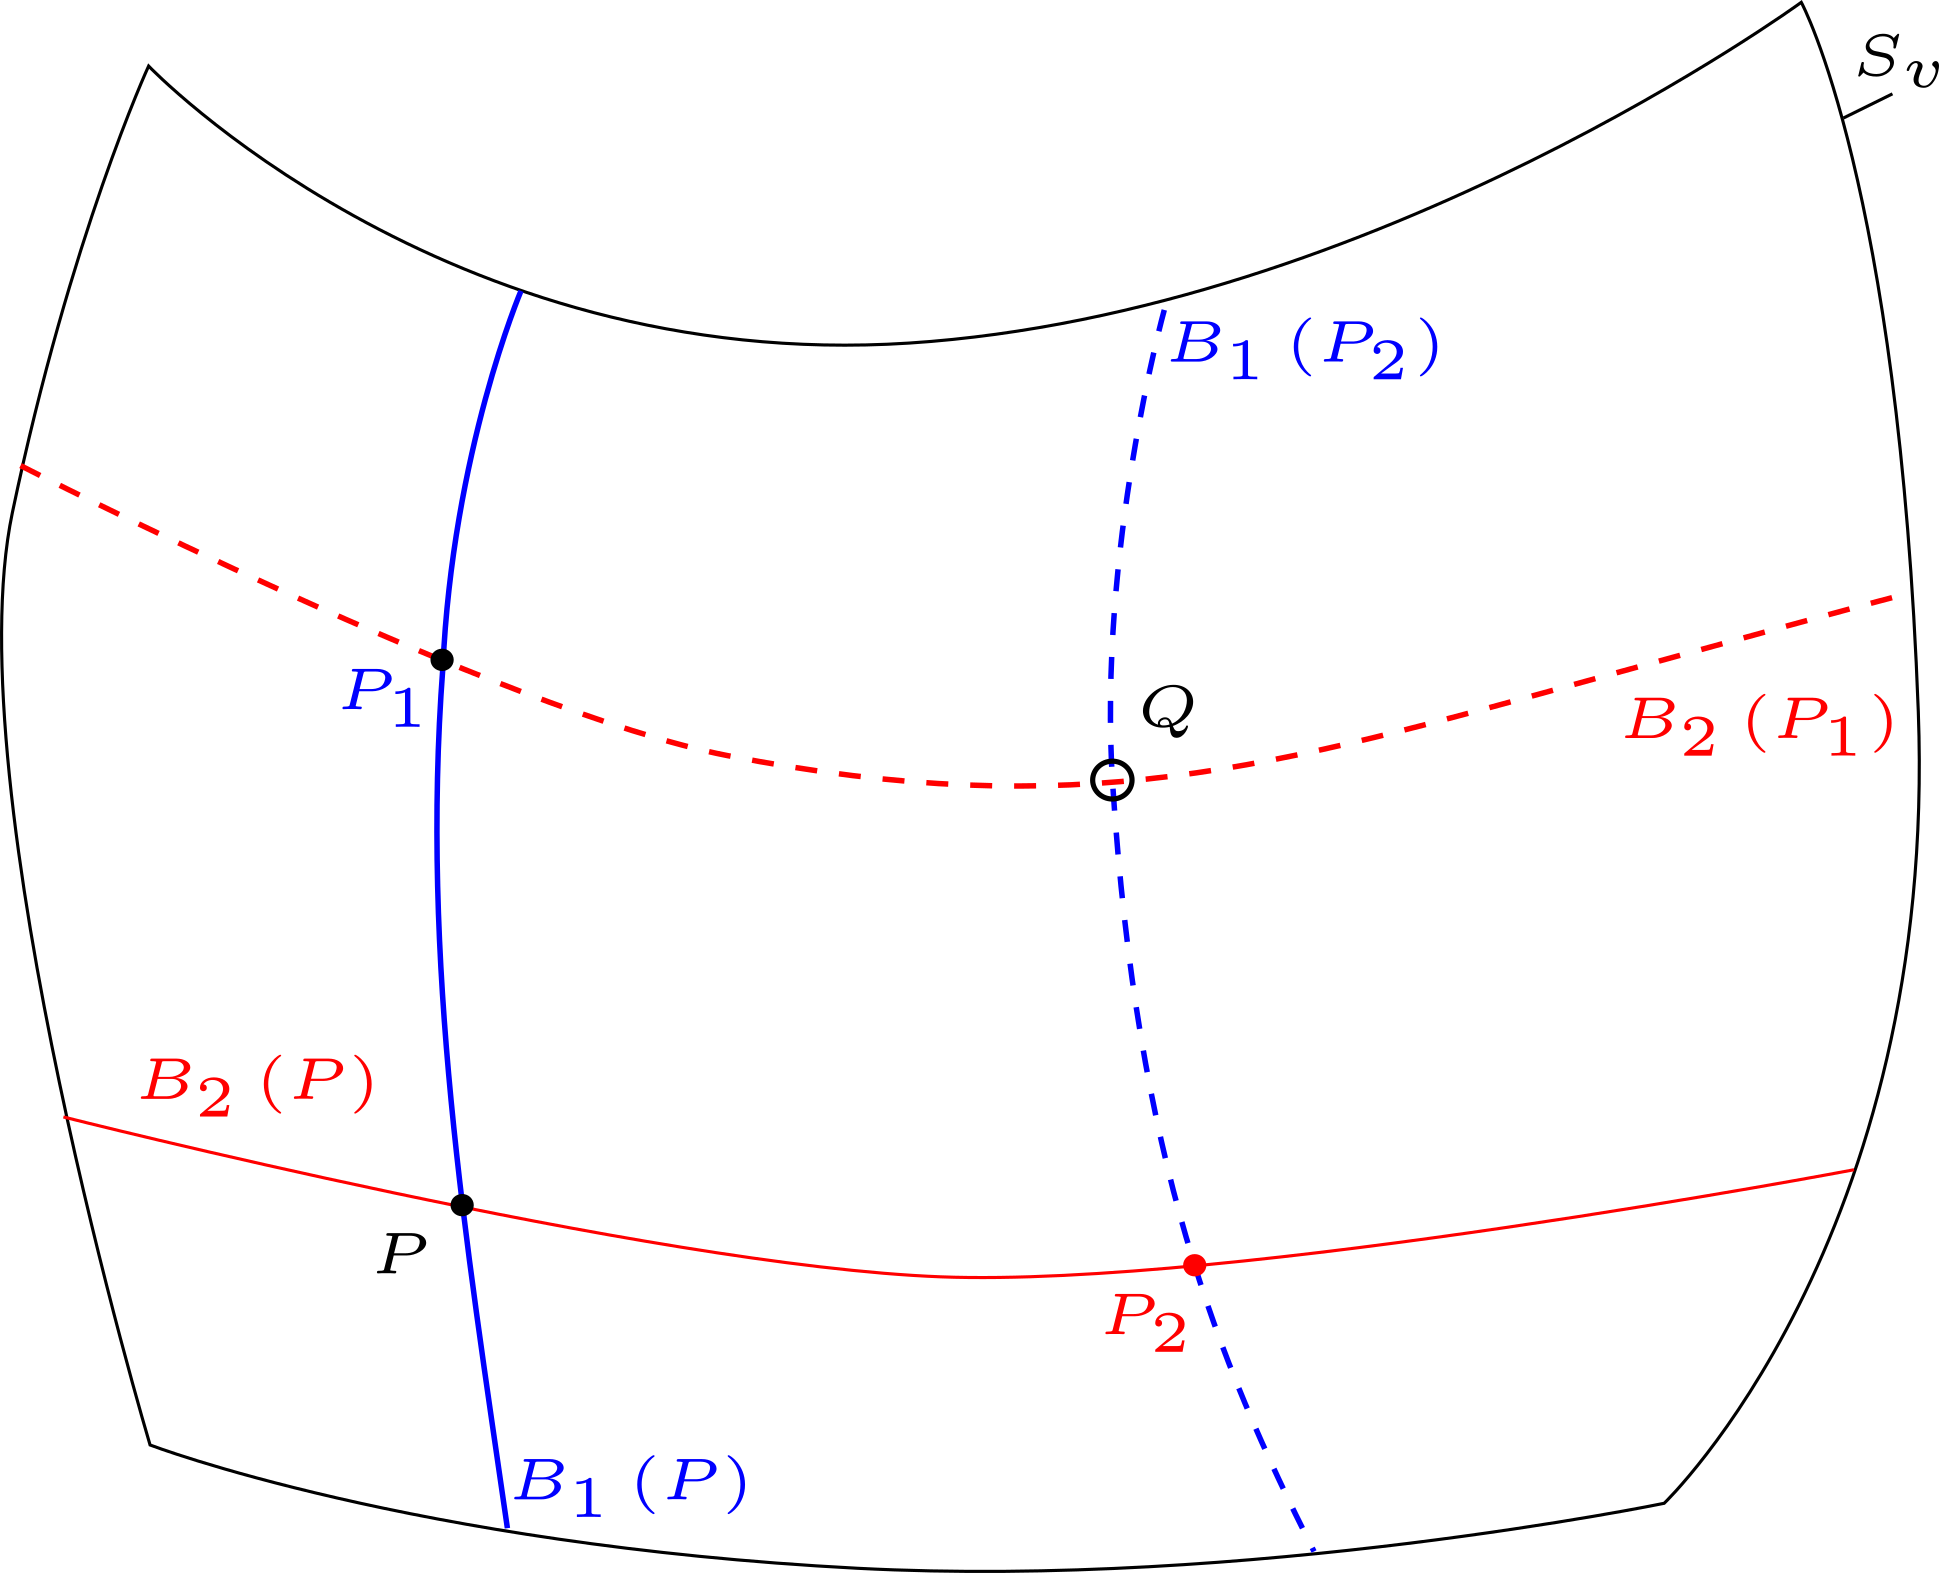
\includegraphics[width=7cm]{FIGS/ClothPathEpip.png} &
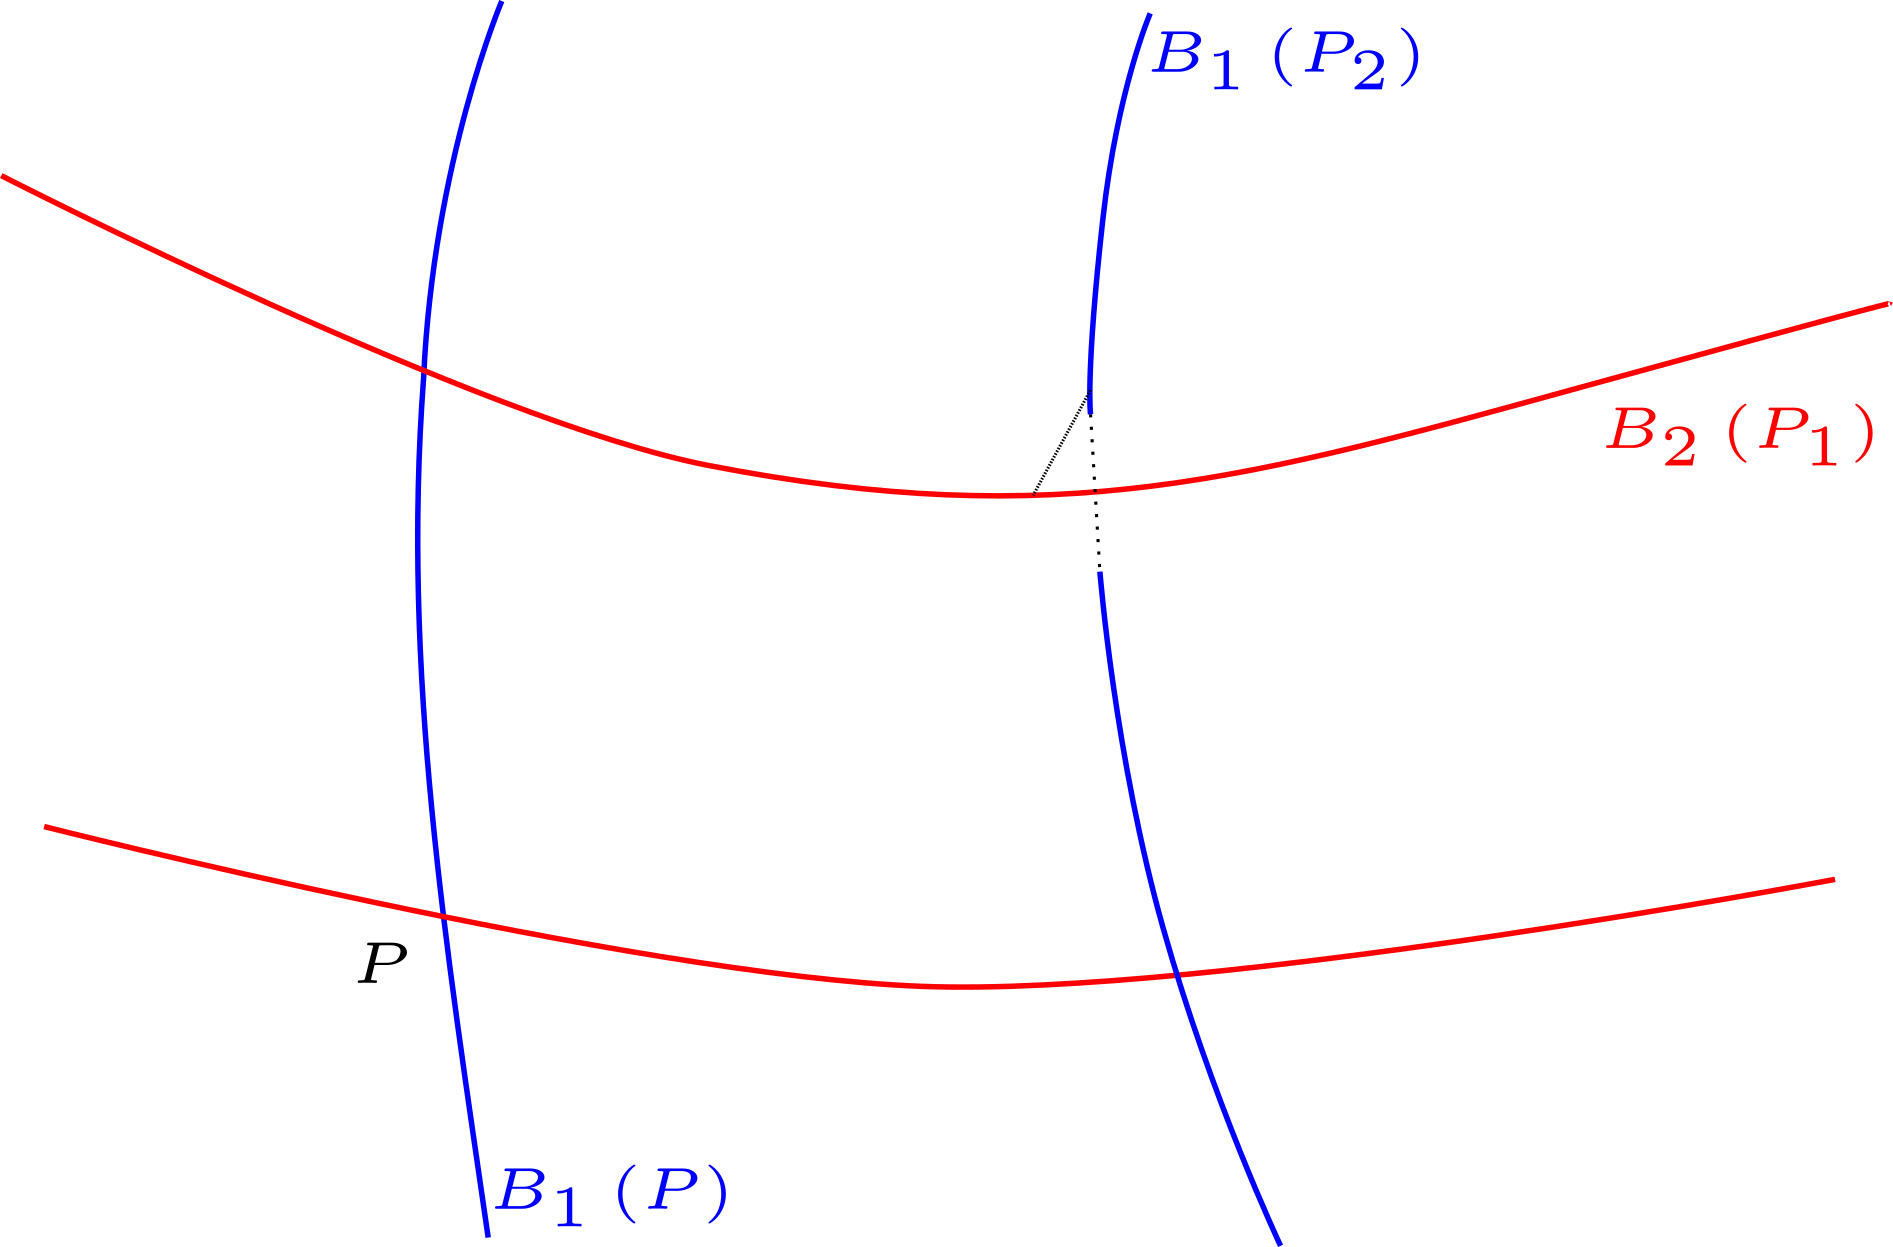
\includegraphics[width=7cm]{FIGS/ClothPathNonEpip.png}\\
% & \\\hline
\end{tabular}
\caption{Path closure. Left: in the epipolar case, the bundles are on the same level of the foliation and the intersection.
Right: in the generic case, the paths don't intersect and no epipolar geometry exists.}
\label{FigClothPath}
\end{figure}

%---------------------------------------------


\subsection{A local characterization of the epipolar existence}

In this section, we derive a local formula (i.e. a differential equation) that measures
the existence of an epipolar geometry. We refer to it as the \textit{epipolarability index}. This section is rather theoretical and
can be omitted by readers mainly interested in practical applications.

Analogously to the proof in Section~\ref{ExistEpip}, we will make a  computation of two-way paths, $\BundO$ then $\BundT$,
as well as $\BundT$ then  $\BundO$. Then, we express the Taylor expansion
of the intersection distance between these two paths. For sake of simplicity, let's suppose that we are in a quasi-vertical acquisition geometry stated in definition \ref{DefQuasiVert}\footnote{Note that we could use
          curvilinear abscissa  when this assumption is not be satisfied.}, and in Figure~\ref{EqDifEpip}, the point $P$ is any point in $\RR^3$. We then denote:
\begin{itemize}
%   \item Make the quasi-vertical assumption \er{tu veux dire acquisition en nadir?} (note that we could use curvilinear abscissa   when this assumption can not  be satisfied);
%   \item Let $P$ be any point in $\RR^3$;
   \item the first path $(P,P_1,Q_1)$ following  $\BundO(P)$ then $\BundT(P_1)$, making a
         progression $\delta_1$ on $\BundO(P)$ and  $\delta_2$ on $\BundT(P_1)$ ;
   \item a second path $(P,P_2,Q_2)$ following  $\BundT(P)$ then $\BundO(P_2)$, making a
         progression $\delta'_2$ on $\BundT(P)$ and  $\delta'_1$ on $\BundO(P_2)$ ;
   \item $\overrightarrow{t_1(P)}=(x,y,1)$ as the tangent to the bundle  $\BundO$  in point $P$
         (and similarly $\overrightarrow{t_2}(P)$);
   \item and write  $\DerPart{F}{z_1}$ to refer to the coordinate system $(i_1,j_1,z) = \PiVert_1^{-1}(x,y,z)$,
         idem for  $\DerPart{F}{z_2}$, and obviously as they are two different coordinate systems, we have in general
        $\DerPart{F}{z_1}  \neq \DerPart{F}{z_2}$.
\end{itemize}

%\mpd{CHANNGEEEEEE    NOTATION DELTA}

%\mpd{CHANNGEEEEEE    NOTATION DELTA}

%\mpd{CHANNGEEEEEE    NOTATION DELTA}


\begin{figure}
\centering
\begin{tabular}{c}
% \hline \\
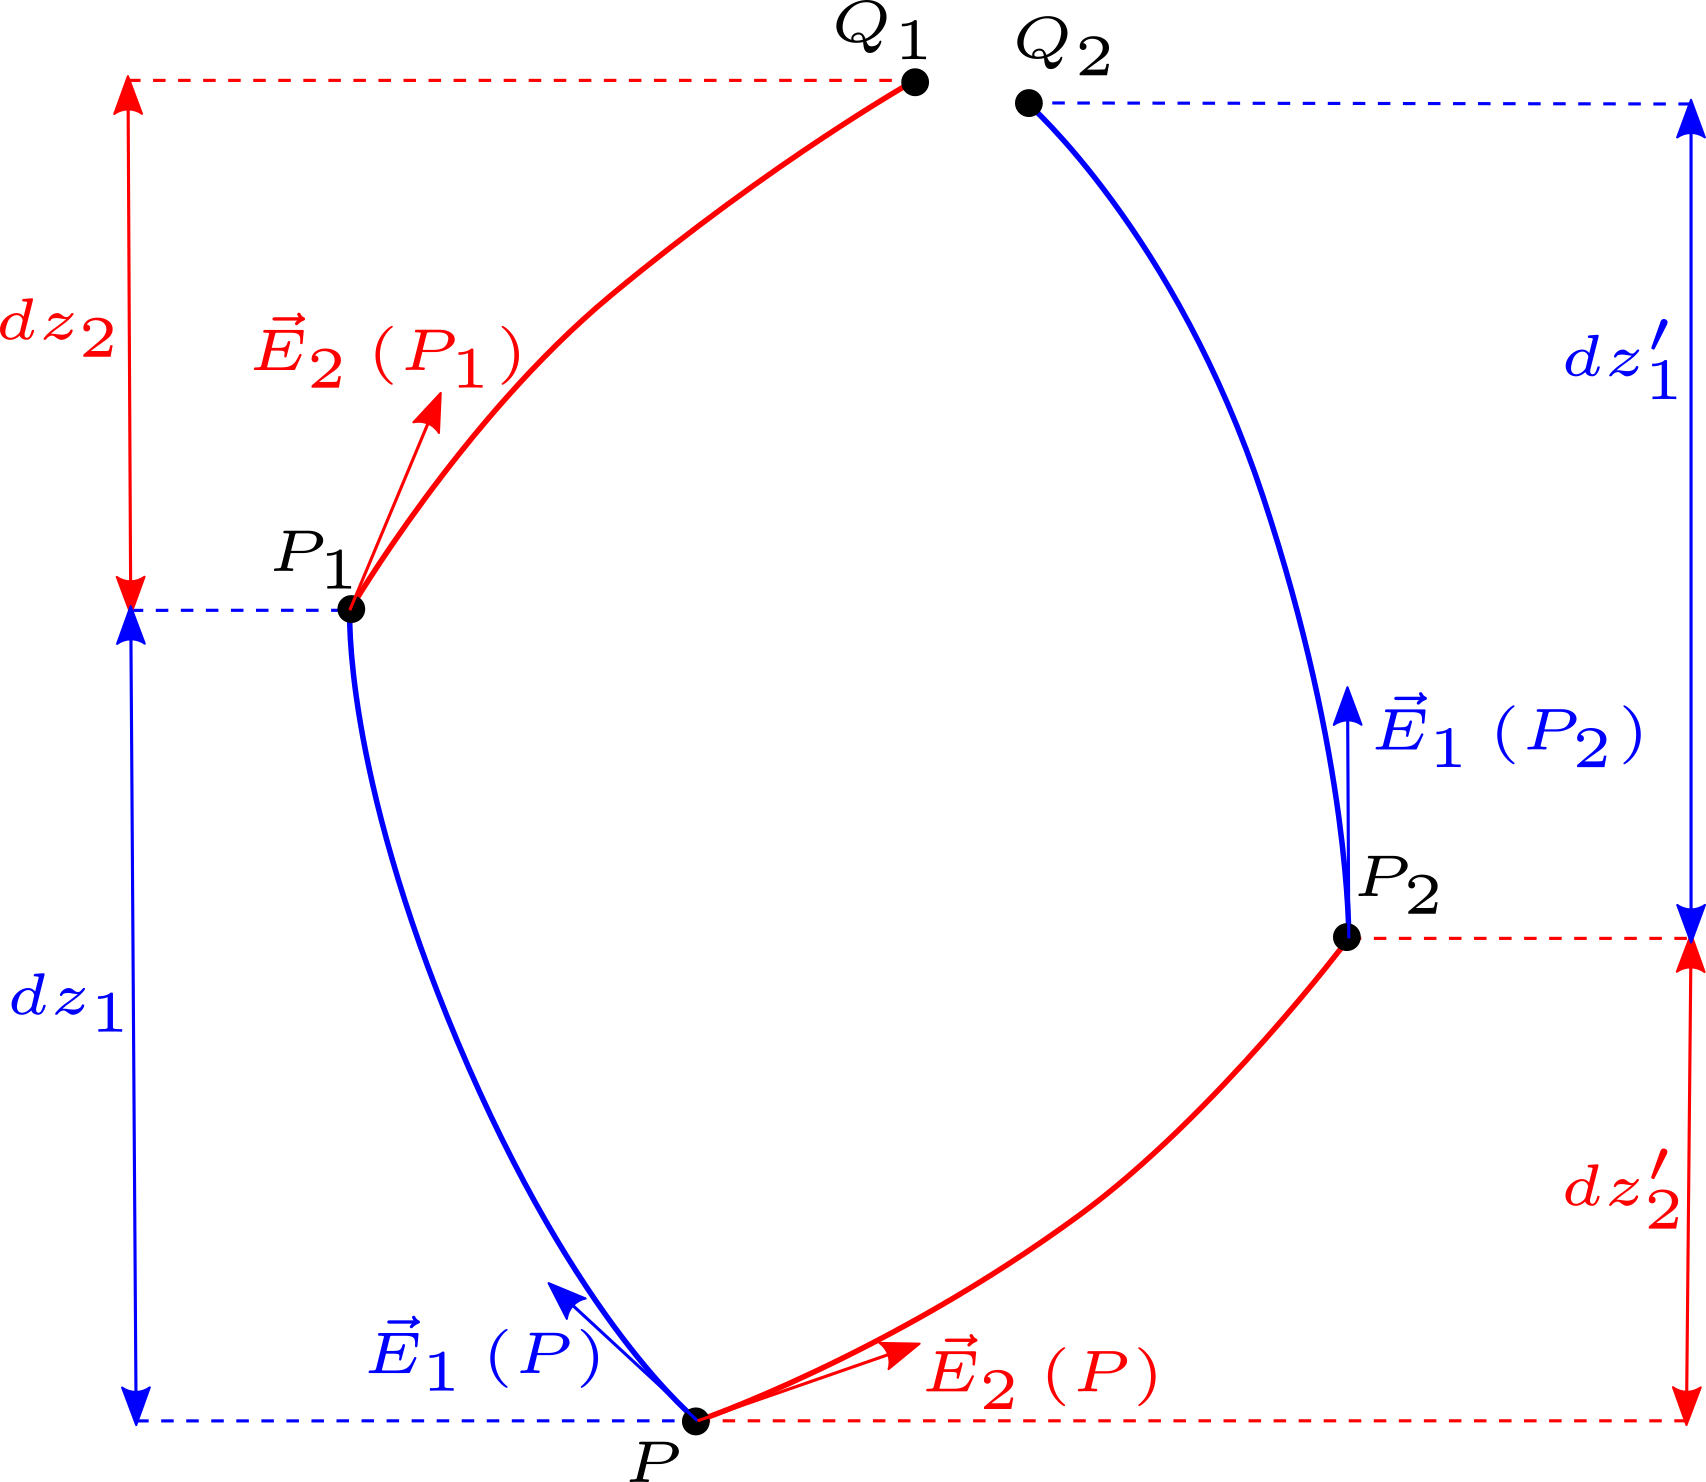
\includegraphics[width=7cm]{FIGS/EquadifEpip.png}
% \\ \\ \hline
\end{tabular}
\caption{Notation for local characterization of the epipolar existence.}
\label{EqDifEpip}
\end{figure}

Now, for any pair of "small" values $(\delta_1,\delta_2)$,  we  compute 
$(\delta'_1,\delta'_2)$ which minimize the distance $|Q_1,Q_2|$ and express the canceling of the
second degree Taylor expansion of this distance (the first degree can always be canceled out as we will see).  Noting $\delta$ the max of all $\delta$, the second degree Taylor expansion gives :

\begin{equation}
    P_1 =  P +  \delta_1 \TanO{(P)} + \frac{{\delta_1}^2}{2} \DerPart { \TanO{}}{z_1}(P)  + \Negl{\delta^3} \label{P1} 
\end{equation}
\begin{equation}
    Q_1 =  P_1 +  \delta_2 \TanT{(P_1)} + \frac{{\delta_2}^2}{2} \DerPart { \TanT{}}{z_2}(P_1) + \Negl{\delta^3} \label{Q1}
\end{equation}
\begin{equation}
     \TanT{(P_1)} = \TanT{(P)} +  \delta_1   \DerPart { \TanT{}}{z_1}(P) + \Negl{\delta^2} \label{TP1}
\end{equation}
%
Putting together Equations~\eqref{P1},~\eqref{Q1},~\eqref{TP1} we can perform a Taylor expansion of the path
$P$ to $Q_1$:
\begin{equation}
    Q_1 =    P +  \delta_1 \TanO{(P)} 
               +  \delta_2 \TanT{(P)} 
               + \frac{{\delta_1}^2}{2} \DerPart { \TanO{}}{z_1}(P) 
               + \frac{{\delta_2}^2}{2} \DerPart { \TanT{}}{z_2}(P) 
               +  \delta_1  \delta_2  \DerPart { \TanT{}}{z_1}(P)  
               + \Negl{\delta^3}
       \label{Q1ofP}
\end{equation}
%
And similarly for $P$ to $Q_2$ :
%
\begin{equation}
    Q_2 =    P +  \delta'_2 \TanT{(P)} 
               +  \delta'_1 \TanO{(P)} 
               + \frac{{\delta'_2}^2}{2} \DerPart { \TanT{}}{z_2}(P) 
               + \frac{{\delta'_1}^2}{2} \DerPart { \TanO{}}{z_1}(P) 
               +  \delta'_1  \delta'_2  \DerPart { \TanO{}}{z_2}(P)  
               + \Negl{\delta^3}
       \label{Q2ofP}
\end{equation}
%
The first degree Taylor expansion of $Q_2-Q_1$ gives :
%
\begin{equation}
    Q_2 -Q_1 =   (\delta'_1 -\delta_1) \TanO{(P)} +  (\delta'_2 -\delta_2) \TanT{(P)}  + \Negl{\delta^2}
\end{equation}
%
To minimize $|Q_2 -Q_1|$, the first step is to cancel the first degree  terms of $ Q_2 -Q_1$. We assume
that $\TanT{(P)}$ and $\TanO{(P)}$  are independant vectors\footnote{Otherwise, it would be a 
degenerate case for stereovision} and we must then make $\delta'_2 -\delta_2$ and $\delta'_1 -\delta_1$ second degree terms:

\begin{equation}
   \Delta_1 =   \delta'_1 -\delta_1 = \Negl{\delta^2}  \; ; \; \Delta_2 =   \delta'_2 -\delta_2 = \Negl{\delta^2}
   \label{Delta}
\end{equation}
%
To develop $ Q_2 -Q_1$ we can use the following identities  that are direct consequences of~Equation~\eqref{Delta}:

\begin{equation}
   \delta_1  \delta_2 -  \delta'_1  \delta'_2  = \Negl{\delta^3} \;;\;
   {\delta_1}^2 - {\delta'_1}^2 =  \Negl{\delta^3} \;;\;
   {\delta_2}^2 - {\delta'_2}^2 =  \Negl{\delta^3} 
   \label{NeglDelta}
\end{equation}
%
Subtracting Equation~\eqref{Q1ofP} from Equation~\eqref{Q2ofP}, and using Equation~\eqref{NeglDelta}, we can write :

\begin{equation}
    Q_2 -Q_1 =   \Delta_1 \TanO{(P)} +   \Delta_2 \TanT{(P)}  
               + \delta_1  \delta_2(\DerPart { \TanT{}}{z_1}(P)  -\DerPart { \TanO{}}{z_2}(P) )
               + \Negl{\delta^3}
\end{equation}
%
We now translate the intersection of paths by canceling the second degree Taylor expansion in $Q_2 -Q_1$. We have three vectors, and their weighted sum can be null iff they are colinear.

\begin{theorem}[Existence of epipolar geometry]
The epipolar geometry exists iff the following determinant is null:

\begin{equation}
\left[ \begin{array}{c|c|c}
\TanO{} & \TanT{}  & \DerPart { \TanT{}}{z_1}  -\DerPart { \TanO{}}{z_2}  
\end{array} \right]  
=0
\end{equation}

\end{theorem}

\begin{remark}[Epipolar equation with central perspective camera]
As an illustration on an easy case, we can see that this condition is trivially 
satisfied for a pair of central perspective cameras as we have the canceling of both terms as shown
in Equation~\eqref{EqEpipConik}. This is because for a given point $P$,
and any point $P_1$ on $\BundO(P)$, $\TanT{(P_1)}$ belongs to the epipolar
plane $\mathcal{P}$. We have $\TanT{(P_1)} \in \mathcal{P}$, so $\DerPart { \TanT{}}{z_1} \in \mathcal{P}$,
and as we have also $\TanO{(P)} \in  \mathcal{P}, \TanT{(P)} \in  \mathcal{P}$, the collinearity
between $\TanO{(P)}$ , $\TanT{(P)}$ and $\DerPart { \TanT{}}{z_1}(P)$ is thus proven:

\begin{equation}
\left[ \begin{array}{c|c|c}
\TanO{} & \TanT{}  & \DerPart { \TanT{}}{z_1}  
\end{array} \right]  
=\left[ \begin{array}{c|c|c}
\TanO{} & \TanT{}  & \DerPart { \TanO{}}{z_2}  
\end{array} \right]  
=0
\label{EqEpipConik}
\end{equation}
\end{remark}


%---------------------------------------------


\subsection{Ambiguity of the epipolar geometry}

When the epipolar geometry exists, the epipolar resampling is not unique. To demonstrate that our rectification method handles this ambiguity rigorously, we first describe it formally.


Let $\phi_1,\phi_2$ and  $\phi'_1,\phi'_2$ be two epipolar resamplings. Following the depiction in Figure~\ref{FigAmbigEpip}, for any $v$, consider the pair of lines $\LineO(v),\LineT(v)$ for which:

\begin{itemize}
   \item  $\phi_k^{-1}(\LineK(v))$ is the curve $\CurveK(v)$ by definition of epipolar resampling;
   \item  and $\phi'_k (\CurveK(v)) = \phi'_k ( \phi_k^{-1}(\LineK(v))$ is a line, also by definition of epipolar resampling;
   \item and in analogy, $\phi'_1 ( \phi_1^{-1}(\LineO(v))) = \phi'_2 ( \phi_2^{-1}(\LineT(v)))$.
\end{itemize}

Consequently we have the following constraints between two pairs of epipolar ressampling:

\begin{itemize}
   \item  $\phi'_1 \phi_1^{-1}$  and $\phi'_2 \phi_2^{-1}$ are diffeomorphisms transforming lines into lines;
   \item $\phi'_1 \phi_1^{-1}$  and $\phi'_2 \phi_2^{-1}$ define the same global transformation on lines
        (i.e. if $\phi'_1 (\phi_1^{-1} (\LineO(v))) = \phi'_2 (i\phi_2^{-1}(\LineT(v)))$).
\end{itemize}


%For any pair of lines $\LineK(v)$ in $E_k$, there are corresponding 
%homologous curves $\CurveO(v),\CurveT(v)$  in images 
%$I_1,I_2$ (see Equation~\eqref{Eq:CurvHom}). Following the depiction in Figure~\ref{FigAmbigEpip}, if $\phi'_k(\CurveK(v)))$
%are  lines $\LineK(v')$ in $E_k$, one can observe that $\phi'_1 \phi_1^{-1}$  and $\phi'_2 \phi_2^{-1}$ are diffeomorphisms transforming lines into lines, and

% they globally aoperate the same transformation on lines
\emph{Vice versa}, let  $\phi_1,\phi_2$ be an epipolar resampling and let $\Lambda_1,\Lambda_2$ 
be diffeomorphisms  that are stable for lines and make globally the same transformation on lines. We can thus note that $\Lambda_1 \circ \phi_1$ and  $\Lambda_2 \circ \phi_2$ are also an epipolar resampling (see Figure~\ref{FigAmbigEpip}).


Having devised the exact ambiguity, we can now define two constraints to impose on a unique epipolar resampling: 
\begin{enumerate}
\item \textbf{Constraint on the uniqueness of the deformation}
inside each line . For instance, one can impose that the colums remain constant (i.e.
the deformation is only made  on  $y$), as given in Equations~\eqref{Ambig:PhiO}
and~\eqref{Ambig:PhiT};
\item \textbf{Constraint on the global deformation} of lines\footnote{i.e. where each line
is transformed globally to another line}. For instance, by fixing the transformation of one image, as given in Equation~\eqref{FigAmbigEpip}.
\end{enumerate}
 

\begin{theorem}[Unique epipolar constraint]

If the epipolar geometry exists, there exists a unique epipolar resampling $\phi_1,\phi_2$ satisfying the  following three constraints:

\begin{equation}
    \phi_1(x,y) = (x,y') \label{Ambig:PhiO}
\end{equation}
\begin{equation}
    \phi_2(x,y) = (x,y') \label{Ambig:PhiT}
\end{equation}
\begin{equation}
    \phi_1(0,y) = (0,y) \label{Ambig:Line}
\end{equation}
\label{Theo:Fix:Ambig}

\end{theorem}

\begin{figure}[h!]
\centering
\begin{tabular}{c}
% \hline \hline
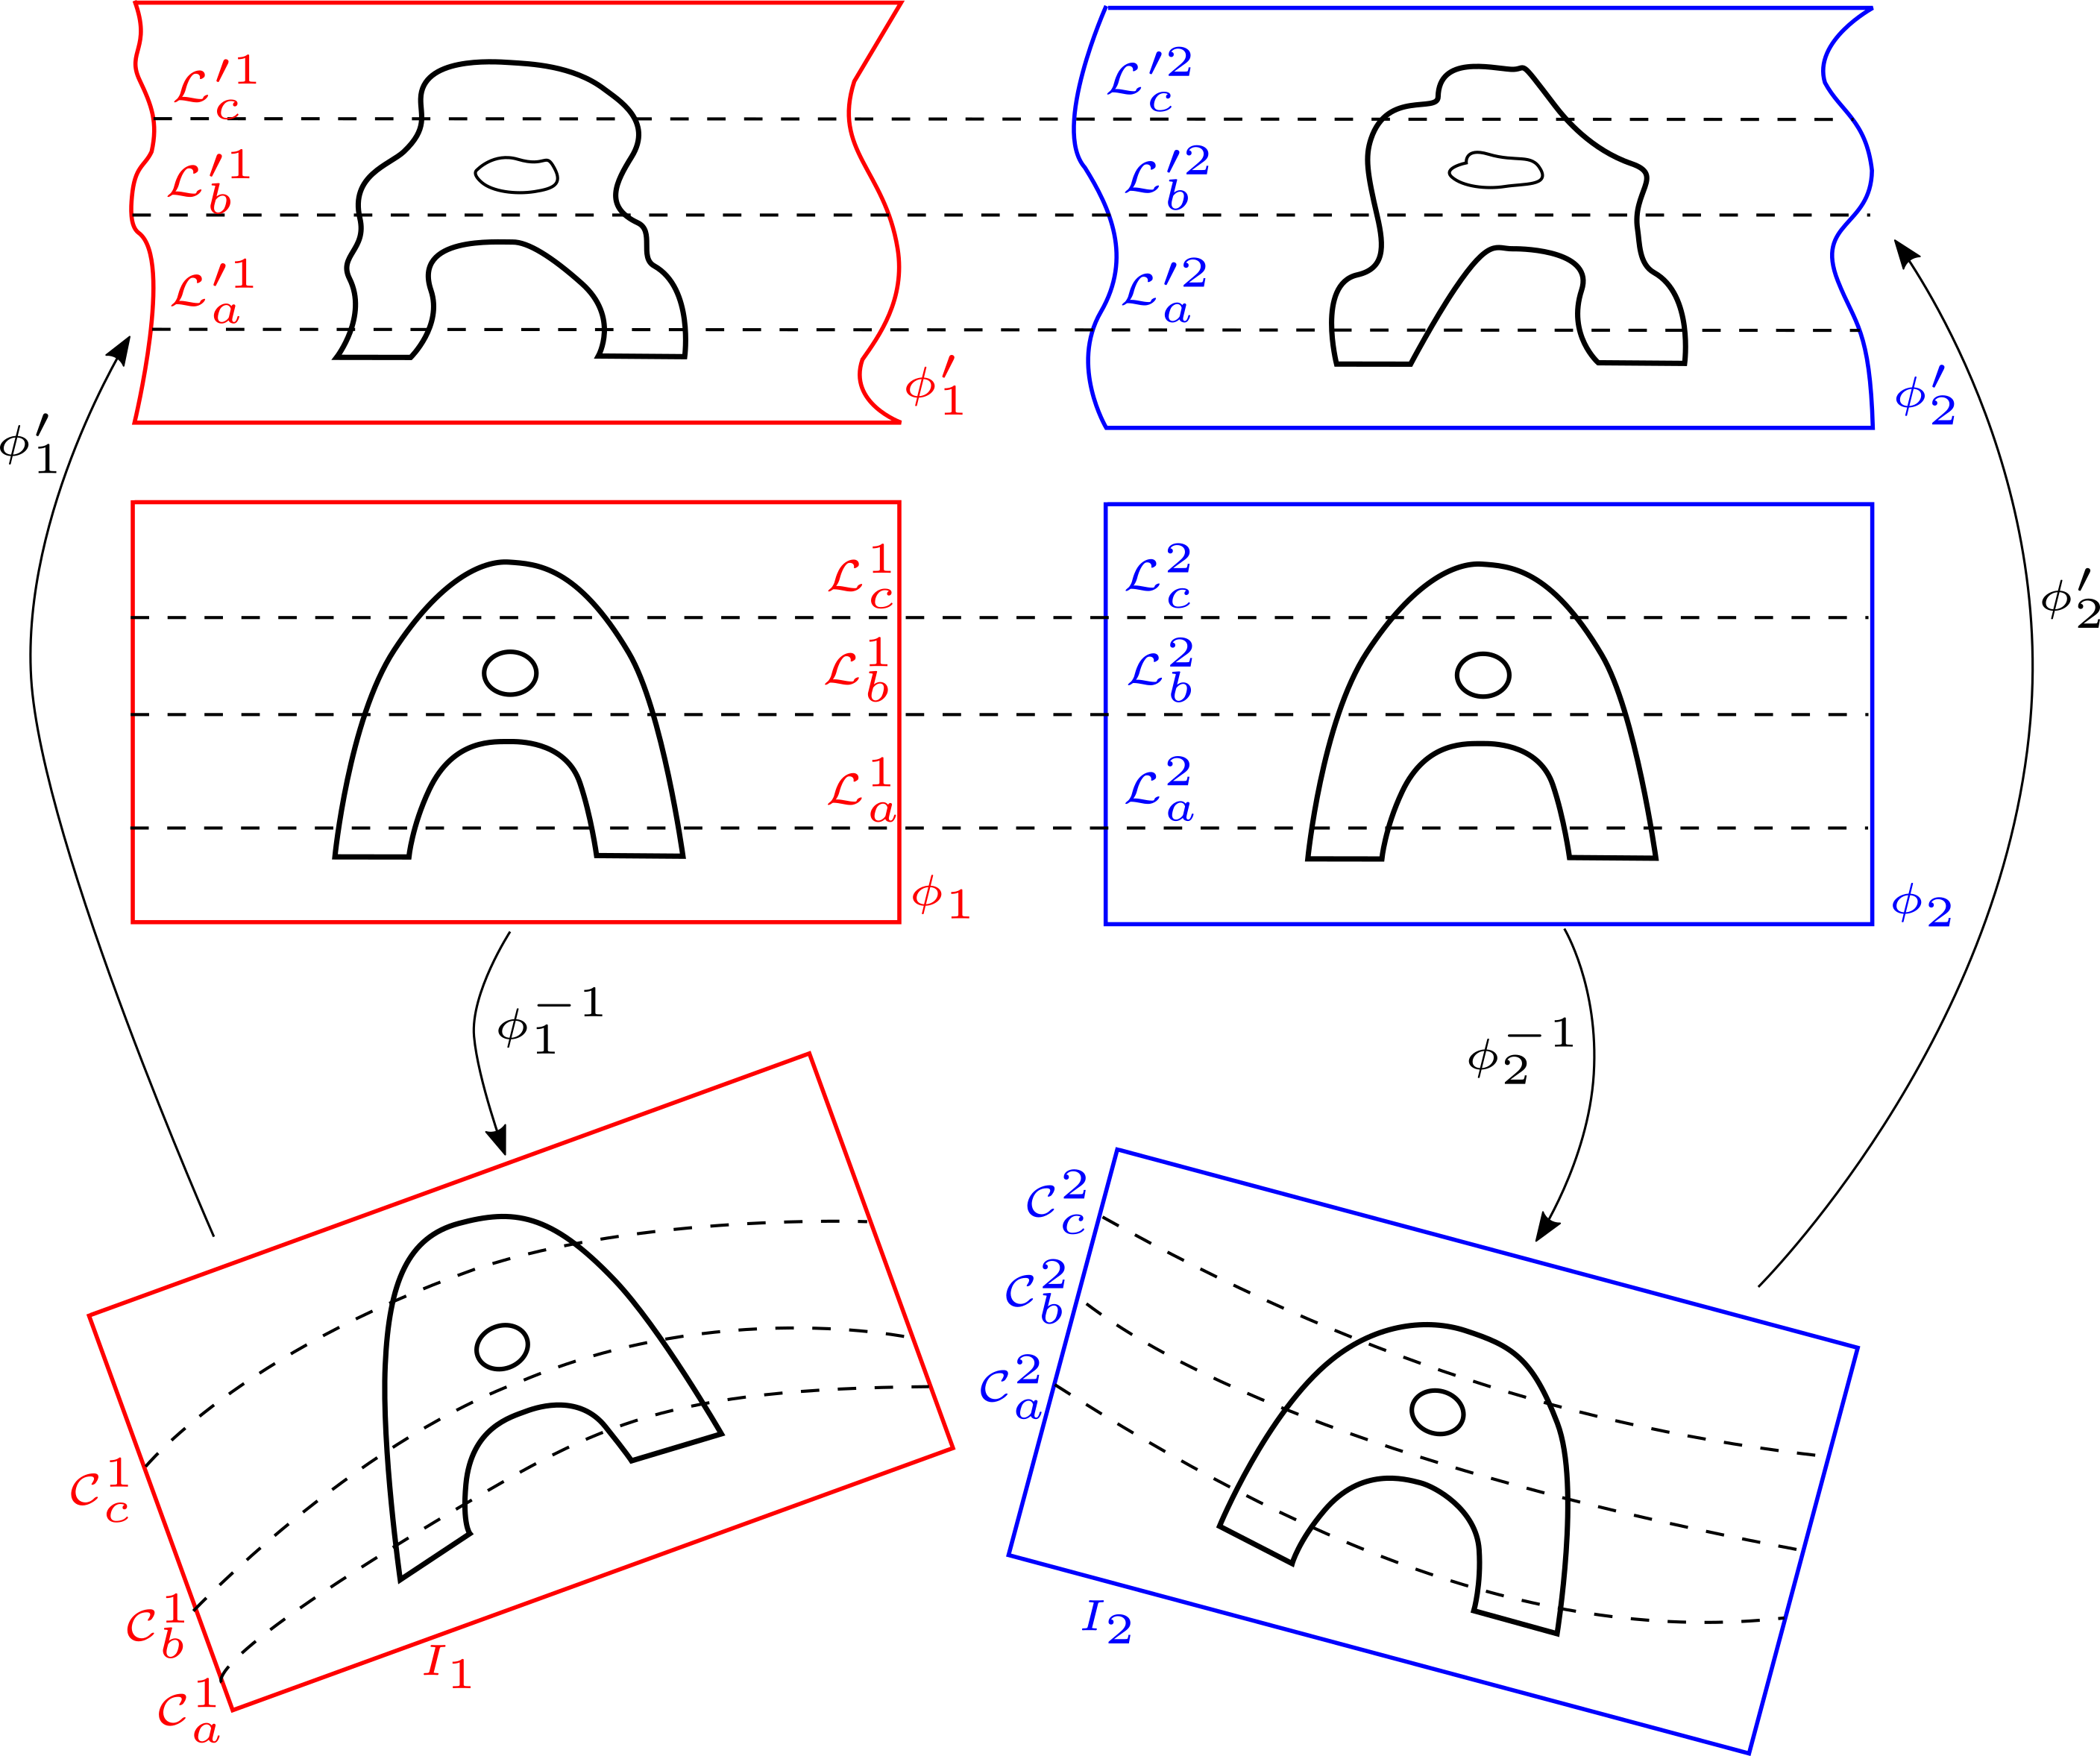
\includegraphics[width=10cm]{FIGS/AmbigEpip.png}
% \\ \hline \hline
\end{tabular}
\caption{Ambiguity of the epipolar geometry: two possible epipolar resamplings for a single stereo pair.}
\label{FigAmbigEpip}
\end{figure}

%---------------------------------------------
%---------------------------------------------
%---------------------------------------------

\section{Proposed method for epipolar geometry resampling}\label{sec:method}


\subsection{Hypothesis and layout}

\subsubsection{Principles}
The principle of the method is to use \emph{H-Compatible}  points $p_1,p_2$ to calculate a
pair of functions $\phi_1,\phi_2$ that comply with the epipolar constraint, i.e. 
\emph{"$\phi_1(p_1)$ and $\phi_2(p_2)$ are on the same line"}. As these epipolar functions
are not unique, we parameterize the $\phi_k$ in Theorem~\ref{Theo:Fix:Ambig}, accordingly:
%
\begin{equation}
    \phi_k(i,j) = (i,V_k(i,j)); \; \;
    V_k : \RR^2 \rightarrow \RR  
  \label{EpipVParam}
\end{equation}
%
This parametrization implements the constraints of Equations~\eqref{Ambig:PhiO} and~\eqref{Ambig:PhiT}. We will account for the constraint of  Equation~\eqref{Ambig:Line} in Section~\ref{ChoicePolyn}. %({see Equations~\eqref{CstrV1:0},~\eqref{CstrV1:1}}). 
To compute $V_1,V_2$, for any pair of \emph{H-Compatible} points, we add an observation that constrains $V_1$ and $V_2$:


\begin{equation}
    V_1(p_1) = V_2(p_2) \label{EqV1V2}.
\end{equation}

\subsubsection{Hypothesis}


The method takes two camera models $\pi_1$ and $\pi_2$ as inputs.
These models are considered black-boxes that satisfy Equation~\eqref{Eq:Proj}, and for which no specific assumption is made on the physical model of the camera. In our \CPP implementation,
the cameras are considered to be pure virtual classes offering the interface to Equation~\eqref{Eq:Proj}.
In this paper, the examples processed by our method are pushbroom satellite models known by their RPCs and the central perspective. However, the only restriction imposed on the generic nature of the model is that the projection function is "smooth", i.e.:

\begin{itemize}
    \item $\pi$ are $\mathcal{C}^{\infty}$ functions, and
    \item the directions of epipolar curves vary within a limited range (for example,
          less than $\frac{\pi}{2}$).
\end{itemize}
%
Figure~\ref{BadGoodEpip} illustrates the latter constraint. The left image presents a set
of epipolar lines with too large direction variations. The right images represent  pairs of epipolar lines whose directions change within a small range, therefore suitable for the proposed resampling method. 
%
\begin{figure}[h!]
\centering
\begin{tabular}{c}
% \hline \hline
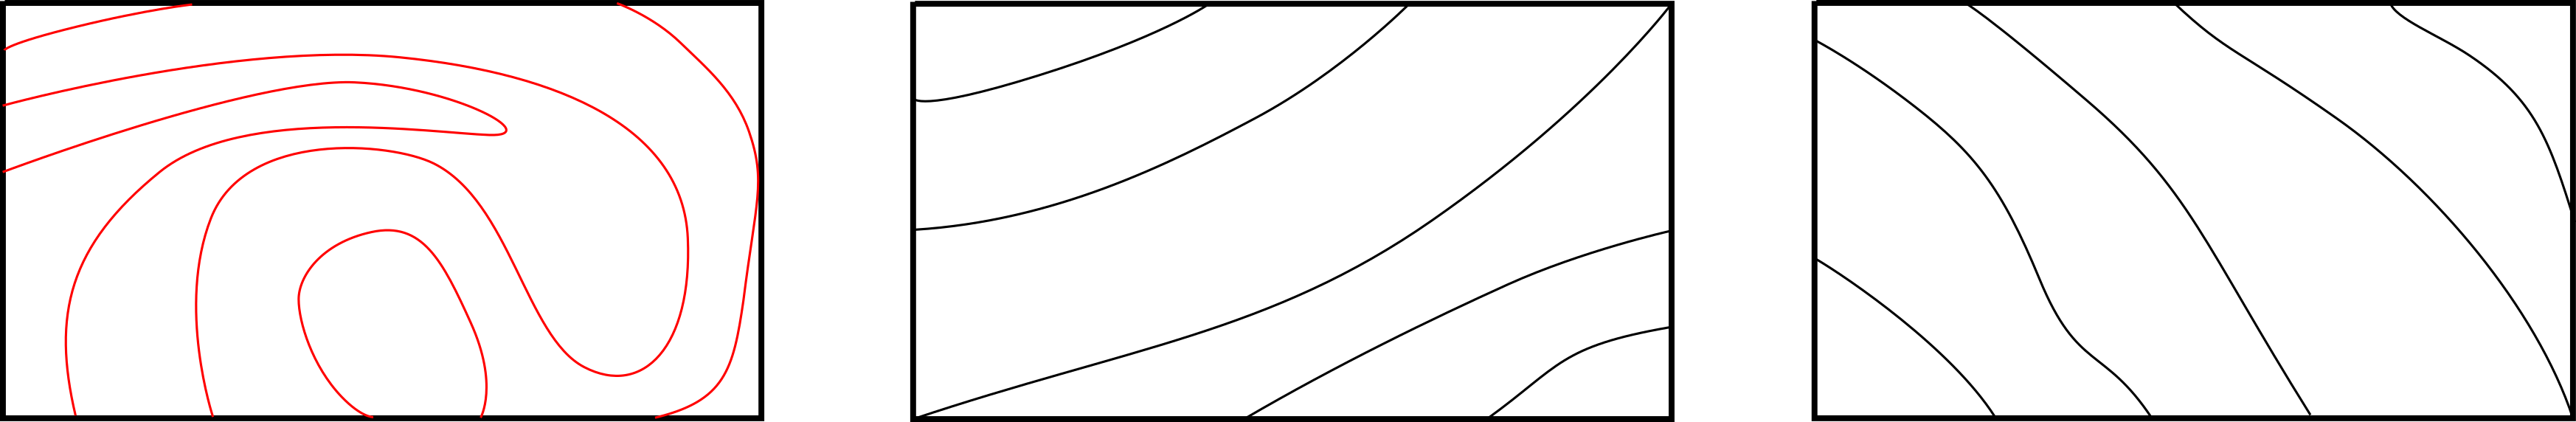
\includegraphics[width=10cm]{FIGS/BadGoodLines.png}
% \\ \hline \hline
\end{tabular}
\caption{Epipolar lines. Left: not handled by our method; Right: acceptable by our method.}
\label{BadGoodEpip}
\end{figure}


\subsubsection{Estimation of the center and the global direction}

\label{EstCenterDir}

Before calculating the rectifying functions $V_k$, we need to compute a coordinate system where epipolar lines are globaly horizontal. This requirement is
a consequence of equation~\eqref{EpipVParam}, and is illustrated by Figure~\ref{ReqOrient}:


\begin{itemize}
   \item The left image of Figure~\ref{ReqOrient} presents a case where epipolar curve are quasi-vertical
         and for which an epipolar correction of Equation~\eqref{EpipVParam}, without an initial rotation,  is impossible;
   \item The center image of Figure~\ref{ReqOrient} presents a case where epipolar curve are slanted;
         In this case epipolar correction according to equation~\eqref{EpipVParam} is possible
         but leads to important distorsion in the image, as can be seen in the image on the right.
\end{itemize}

\begin{figure}
\centering
\begin{tabular}{c}
% \hline \hline
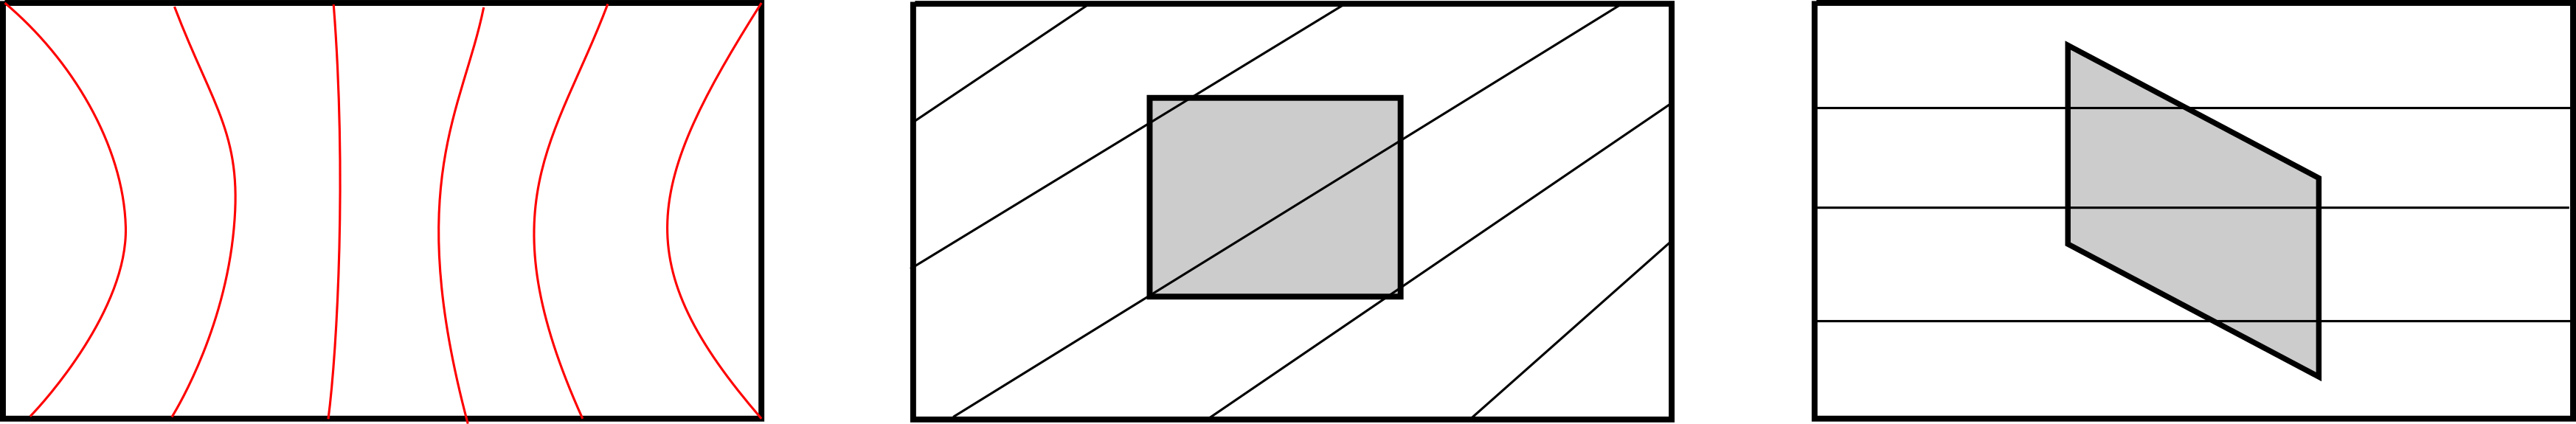
\includegraphics[width=10cm]{FIGS/EpipReqOrient.png}
% \\ \hline \hline
\end{tabular}
\caption{Left: Quasi-vertical epipolar curve for which correction with Equation~\eqref{EpipVParam} is impossible.  Middle and right: slanted curves for which epipolar rectification  with Equation~\eqref{EpipVParam} is possible
         but generates significant distortion.}
\label{ReqOrient}
\end{figure}

Therefore, for each image we estimate the average direction $\vec{D}_k$
of their epipolar lines, and a rotation $R_k$ is applied on the  input set of points $p$:

\begin{equation}
    R_k(p) =  \frac{p-C_k}{\vec{D}_k},  \label{EqRot}
\end{equation}

where $C_k$ is the centroid of the set of points. The epipolar lines are now globally horizontal and the subsequent epipolar deformation is computed on the rotated data points. 

%To begin with, the method estimates the centers  $C_1,C_2$ of a set of points $p_1$ and $p_2$. This is done by calculating the average of all points' coordinates.  Then, the computations continue in the coordinate systems centered at $C_1,C_2$. After this "normalisation", the constraint in Equation~\ref{Ambig:Line} is applied at these centers.


\subsubsection{Layout}

The layout of the method follows three steps: (1) estimate the global 
direction of epipolar lines; (2) estimate $F_1,F_2$ as  the local epipolar rectification
 in the coordinate system linked to the global direction; (3)  estimate the final
epipolar rectification as a composition of $F_1,F_2$ and the rotation.
A more formalized description of the algorithm is given in Algorithm~\ref{AlgoGlob}.


\begin{algorithm}[H]
\caption{Epipolar($\pi_1$,$\pi_2$). \emph{Layout of the algorithm for computing the epipolar rectification from camera models}}
\begin{algorithmic}
   % \STATE {\emph{Layout of the algorithm for computing the epipolar rectification from camera models}}
    \STATE Use $\pi_1,\pi_2$ to estimate a set of \emph{H-Compatible} points $\mathcal{H} =\{(p_1,p_2)\}$ : 
    \STATE Estimate centers $C_1$ and $C_2$;
    \STATE Estimate global direction of epipolars $\vec{D}_1$ and $\vec{D}_2$,
    \STATE Estimate rotations $R_1,R_2$ according to Equation~\eqref{EqRot}
    \FORALL{$p_1,p_2 \in \mathcal{H}$}
              \STATE set: $q_1 = R_1(p_1)$,  $q_2 = R_2(p_2)$
              \STATE add equation: $V_1(q_1) = V_2(q_2)$
    \ENDFOR
    \STATE estimate with the least squares method $V_1$ and $V_2$
    \STATE set $F_k(x,y)=(x,V_k(x,y))$  %, $F_2(x,y)=(x,V_2(x,y))$
    \STATE set $\phi_k =  F_k \circ  R_k $ % and $\phi_2=F_2 \circ R_2$
    \RETURN $(\phi_1,\phi_2)$
\end{algorithmic}
\label{AlgoGlob}
\end{algorithm}



\subsubsection{Why does our method work?}
\label{WhyWork}

Intuitively, it may not be  obvious that the system of equations in Equation~\eqref{EqV1V2} is well posed.
In fact, if there was a functional relationship between
$p_1$ and $p_2$, as $p_1=F(p_2)$,  an infinity of solutions
for $(V_1,V_2)$ would exist, because   for any function $V: \RR^2 \rightarrow \RR $ we can generate a solution $(V,V\circ F)$.

However, note that due to {the $3$D aspect} of $p_1$ and $p_2$, there is
\emph{no} functional relationship between them which conduct to a more constrained system
of equations. Instead of a functional relationship,
we can generate  "one to many" (and  "many to one") correspondences as illustrated in Figure~\ref{NonFuncCorresp}.
For example, for a given  point $p_1$, following the curve $\pi_2(\BundO(p_1))$, we can generate
several points on the bundle (potentially an infinity) which results in many correspondences.
%by  $\pi_2$ for a single point. 
To illustrate, if we take $p^k_2$ to be $k$ homologous points of $p_1$,
we then have the equation:
%
\begin{equation}
    V_1(p_1) = V_2(p^1_2)   \;;\; V_1(p_1) = V_2(p^2_2)   \;;\; V_1(p_1) = V_2(p^3_2)  \dots , \label{MultiTieP}
\end{equation}
%
which in fact enforces this constraint: 
%
\begin{equation}
V_2(p^1_2) = V_2(p^2_2)  =  V_2(p^3_2) \dots \label{RedrCurv}
\end{equation}
%
If we now look at left image of Figure~\ref{NonFuncCorresp}, we see that Equation~\eqref{RedrCurv}
imposes the constraint that a "piece of curve" is horizontal.
In Section~\ref{EpipTieP}, we will see a more detailed analysis explaining how the 
method can work even with configurations different than those depicted in Figure~\ref{NonFuncCorresp}.


\begin{figure}[h!]
\centering
\begin{tabular}{c}
% \hline \hline
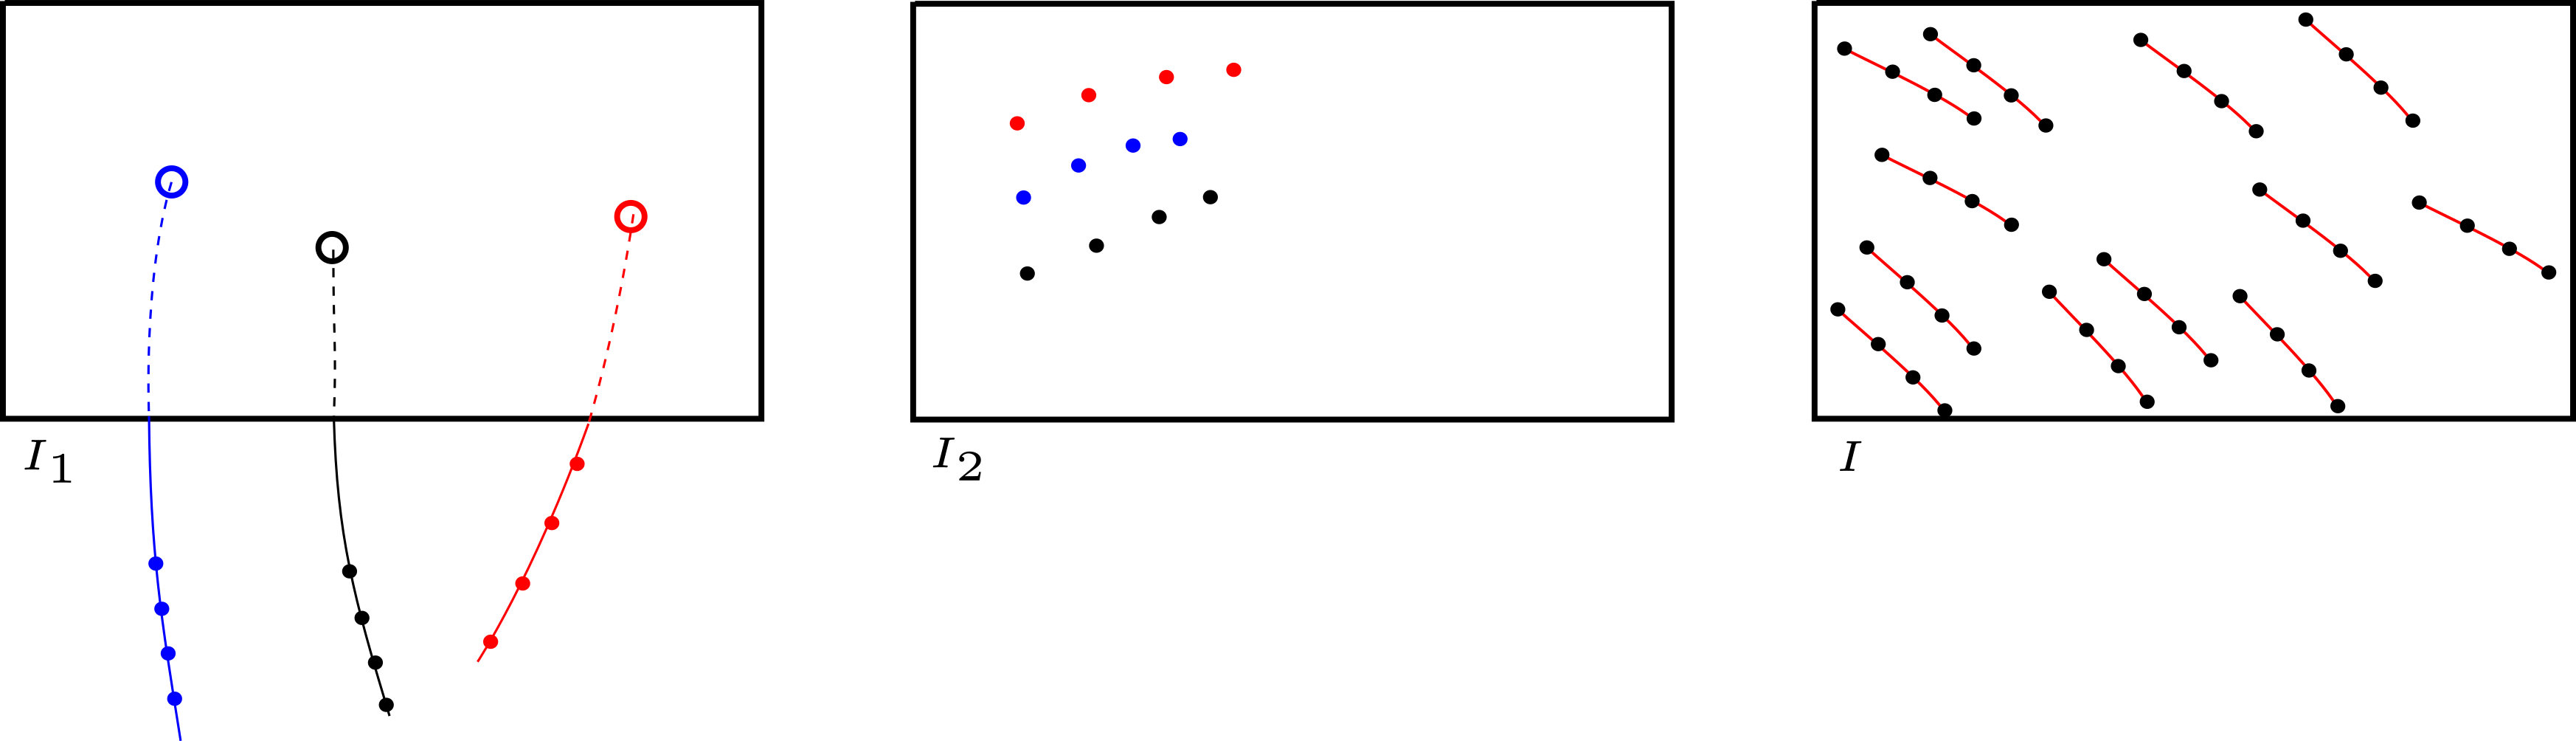
\includegraphics[width=10cm]{FIGS/NonFuncCorresp.png}
% \\ \hline \hline
\end{tabular}
\caption{Left: For each $p_1$, we generate several $3$D points on $B_1(p_1)$. Middle:
         The multiple correspondences in $I_2$. Right: A dense network of curves in $I_2$.}
 
\label{NonFuncCorresp}
\end{figure}

%---------------------------------------------
%---------------------------------------------
%---------------------------------------------


\subsection{Detailed implementation}\label{subsec:implement}


\subsubsection{Choice of a parametric functional space}
\label{ChoicePolyn}

We need to select a space of parametric functions to represent $V_1,V_2$. The only constraint
is that $V_1,V_2$ are $\mathcal{C}^{\infty}$ functions, and that the additional constraint in 
Equation~\eqref{Ambig:Line} is valid. 

Classically, when parameterizing a set of functions  $\mathcal{C}^{\infty}$,
a "natural" candidate is the set of polynomials of a given degree. We know that the function will be
$\mathcal{C}^{\infty}$ and, according to the Stone-Weierstrass theorem \cite{Weierstrass1885,Stone1937} (which says that the space of polynomials is dense in the space of continuous functions),  with a sufficiently high
degree we will be able to accurately approximate any continuous function. A~possible
limitation of selecting high degree polynomial is over-fitting, which may lead to
unwanted high frequency behavior. In our case, this problem should never arise as the measurements  are synthesized from the projection functions $\pi_1,\pi_2$, which provides sufficient redundancy (for instance,
 hundreds of times more measurements than constraints). {Note, however, that some precautions must be taken with respect to the polynomial degree when using our method with image correspondences, without the geometric model (see Section~\ref{EpipTieP})}.

If $d$ is the selected degree, the two vectors of unknowns $C^1_{a,b},C^2_{a,b}$, 
corresponding to coefficients of the polynomials are:


\begin{equation}
   V_k(p) = V_k(i,j) =  \sum\limits_{\substack{a=0}}^d  \sum\limits_{\substack{b=0}}^{d-a}  C^k_{a,b}  i^a j^b. \label{EqPol}
\end{equation}
   
\subsubsection{Imposing constraints on global lines deformation}

%In this paramatrisation, we must take into account Equation~\eqref{Ambig:Line}.
{When applying the constraint of equation~\eqref{Ambig:Line} to equation~\eqref{EqPol}, 
we have $i=0$, hence we can suppress all terms  $i^a$ for $a\neq 0$}. The constraint equation then reads:

\begin{equation}
    V_1(0,j) =  j =   \sum\limits_{\substack{b=0}}^{N}  C^1_{0,b}  j^b  \label{CstrV1:0}
\end{equation}

In the equation above, $j$ on the left and the  sum on the right are both polynomials. If the two polynoms are equal on a interval, their coefficient must be equal . This constraint fixes the $C^1_{0,k}$ : $C^1_{0,1}=1$ and $C^1_{0,k}=0$ otherwise.
%The constraint then comes to force a number the unknowns $C^1_{0,k}$ which have known values: $1$ for $C^1_{0,1}$ and $0$ otherwise.
Using the Kronecker delta, we can write:

\begin{equation}
         C^1_{0,k} = \delta_{1,k} \label{CstrV1:1}
\end{equation}

\subsubsection{Generation of points, computation of the direction and centers}

The  points from $\pi_1$ and $\pi_2$ are generated twice, using each image as the master. The bundles are always generated from the  master images. The Algorithm~\ref{AlgoGenData} presents the 
generation of the points with $I_1$  as the master, as well as the computation of the global direction and the points' centers.

\begin{algorithm}[H]
%\emph{Compute a list $L_{1,2}$  of   $\pi_1-\pi_2$ H-compatible pair with $I_1$ as master image,  compute also center $c_1$ of points of $I_1$  and global direction $\vec{D}_2$ for epipolar curves of $I_2$}
\caption{GenerateData(). \emph{Compute a list $L_{1,2}$  of   $\pi_1-\pi_2$ H-compatible pairs with $I_1$ as the master image.
 Compute also the center $C_1$ of points in $I_1$  and the global direction $\vec{D}_2$ for epipolar curves of $I_2$.}}
\begin{algorithmic}
    \STATE $L_{1,2}\gets () $ ;  $C_1 \gets (0,0)$  ;   $\vec{D}_2 \gets  \overrightarrow{(0,0)}$ ; $N \gets 0 $
    \FOR{$p_1.x=0$  \TO $X_1$  {\bf Step} $\delta_{x,y}$   } 
        \FOR{$p_1.y=0$  \TO $Y_1$  {\bf Step} $\delta_{x,y}$    } 
             \FOR{$z=Z_0$  \TO $Z_1$  {\bf Step} $\delta_{z}$   } 
                  \STATE {$p_2 = \pi_2(\PiVert^{-1}_1(p_1,Z))$}
                  \STATE {$p'_2 = \pi_2(\PiVert^{-1}_1(p_1,Z+\delta_{z}))$}
                  \IF {$p_2 \in I_2$ \AND $p'_2 \in I_2$}
                       \STATE $L_{1,2}.append((p_1,p_2))$  
                       \STATE $C_1 \gets C_1 + p_1$
                       \STATE $\vec{D}_2 \gets  \vec{D}_2 + \frac{\overrightarrow{p_2 p'_2}}{|p_2 p'_2|}$
                       \STATE $N \gets  N +1 $
                  \ENDIF
             \ENDFOR
        \ENDFOR
    \ENDFOR
    $C_1 \gets \frac{C_1}{N}$  ; $\vec{D}_2 \gets \frac{\vec{D}_2}{N} $
\end{algorithmic}
\label{AlgoGenData}
\end{algorithm}


%  \er{what is it? \ref{PiInvert}}
%\paragraph{Using center and direction}

Once the centers $C_1,C_2$, directions   $\vec{D}_1,\vec{D}_2$  and the list $L_{1,2}$ are computed,
they are used to normalize the measurements and make the direction globally
horizontal by applying Equation~\eqref{EqRot} to all elements of the list.


\subsubsection{Estimating the rectification}

As the measurements are synthetic and without outliers, we can directly solve
the equations with the linear least squares  method. Let's sum up all previous steps. Let $d$ be the degree of the polynomials, and the unknowns are the coefficient of the polynomials $V_1$ and $V_2$. There are
          $\frac{(d+1)(d+2)}{2}$ unknowns for $V_2$ and $\frac{(d+1)(d+2)}{2}-(d+1) $  for $V_1$,
          taking into account the  constraint in Equation~\eqref{CstrV1:1}. For each pair of normalized points $q_1,q_2$ (see Algorithm~\ref{AlgoGlob}) we add 
          the Equation~\eqref{EqPol} to the least squares equation system. We then estimate the $V_1,V_2$ and obtain:
%
\begin{equation}
  \varphi_k(p) = \varphi_k(i,j) = (i,V_k(i,j))  \;;\;    \phi_k =  \varphi_k  \circ R_k 
\end{equation} 
%


\paragraph{Estimating the inverse function}

The natural way to resample  $I_k$ in $E_k$ (see Figure~\ref{FigNotaComp}) is to write:

\begin{equation}
  E_k(p) = I_k(\phi^{-1}_k(p)).
\end{equation}
Therefore, to rectify an image, we also need to calculate the inverse function. The inverse of $R_k$ is obvious. For computing the inverse of $\varphi_k$,  we
exploit the fact that if $\varphi$ is invariant for the column, then $\varphi^{-1}$ is invariant too. Consequently, we can parametrize it with a function $W: \RR^2 \rightarrow \RR$ as:

\begin{equation}
  \varphi^{-1}_k(p) = \varphi^{-1}_k(u,v) = (u,W_k(u,v))  
\end{equation}
%
To estimate  $W$, we follow the same rationale as in Section~\ref{ChoicePolyn}, and
use the base of a polynomial function. Once the $V_k$ are known, we generate
for each point $p_k=(i,j)$ in $L_{1,2}$ an observation:

\begin{equation}
   W_k(i,V_k(i,j))  = j \label{InverseEpip}
\end{equation}

If we want to ensure that the computed inverse is sufficiently close
to the "real" inverse, we can increase the polynomial's degree (in our implementation, we typically use the degree of $d+4$). It has no side effects as long as we maintain high redundancy.

%---------------------------------------------
%---------------------------------------------
%---------------------------------------------


\subsection{Epipolar resampling without the geometric model}
\label{SecEpipNoModel}

\subsubsection{Resampling with image correspondences only}

\label{EpipTieP}

\emph{"Is it possible to use
the proposed method to compute the epipolar geometry
if we have image point correspondences (i.e., image features) between the image pairs but we don't know their geometric models?"} There is {NO}
 straightforward answer to whether it is possible or not. In general, it is not possible,
but it becomes possible when the relief (i.e., the 3D scene) is not smooth and we constraint the resampling be more or less smooth.
 %As elaborated in the following pros and cons arguments, the
 % answer depends on the point correspondences, 
%  and is a trade-off between the nature of the 3D scene and the complexity of the model. 
%In fact there is \er{easy yes/no answer as there pro and cons arguments to solve this question} and, as we will see, the precise answer depends of the tie points (it is in fact a trade-off between the nature of the relief and complexity of the model).
%

The rationale behind trying to use exclusively image correspondences comes directly from Algorithm~\ref{AlgoGlob}. As one can see, it does not matter if the point correspondences are extracted with the help of some geometric model (as with Algorithm~\ref{AlgoGenData}) or from an image processing method not requiring any
\emph{a priori} information on image geometry, e.g. SIFT \cite{lowe2004distinctive}. Hence, as long as we know the directions of the epipolar lines, our method is applicable.

However, when the point correspondences are computed with an image processing routine,
 there exists some functional relationship between them. Suppose that the 3D scene can be described by a function $Z=\mathcal{Z}(X,Y)$, and denote $S^\mathcal{Z}$ as the corresponding surface. For a point $p_1$ of $I_1$, denote $ \PiZVert (p_1)$ as the intersection of  $\BundO(p_1)$ and the surface  $S^\mathcal{Z}$. Here, the function $\PiZVert$ is the inverse of the projection  $\pi_1$ which relates the image $I_1$ and the surface $S^\mathcal{Z}$. We now see that there exists a functional relationship between all the point correspondences $(p_1,p_2)$ and it follows this equation:
\begin{equation}
   p_2 = (\pi_2 \circ  \PiZVert) (p_1) = F^\mathcal{Z}(p_1).
\end{equation}
Therefore, as discussed in Section~\ref{WhyWork}, in the most general
case, it is impossible to recover the epipolar geometry from a set of correspondences.
%
%{\underline {\bf Pro:}}  Algorithm~\ref{AlgoGlob} uses only point correspondences and a direction to compute the epipolar geometry. It does not matter if the point correspondences are extracted from the geometric model (as with Algorithm~\ref{AlgoGenData}) or from an image  processing method, e.g. SIFT \cite{lowe2004distinctive}, which does not require any \emph{a priori} information on image geometry. Hence, as long as  we know the directions, our method can be used.


%{\underline {\bf Cons:}} When the point correspondences are computed with an image processing routine, there exists some functional relationship between them. Suppose that:

%\begin{itemize}
%   \item The 3D scene can be described by a function $Z=\mathcal{Z}(X,Y)$,
%         and denote $S^\mathcal{Z}$ as the corresponding surface;
%   \item For a point $p_1$ of $I_1$, denote $ \PiZVert (p_1)$
%         as the intersection of  $\BundO(p_1)$ and the surface  $S^\mathcal{Z}$;
%         $\PiZVert$ is the inverse of the projection  $\pi_1$ 
%         which relates the image $I_1$ and the surface $S^\mathcal{Z}$.
%\end{itemize}
%We now see that there exists a functional relationship between all the point correspondences $(p_1,p_2)$ and it follows the equation:
%\begin{equation}
%   p_2 = (\pi_2 \circ  \PiZVert) (p_1) = F^\mathcal{Z}(p_1).
%\end{equation}
%
% when there is a functional relation $p_2=F(p_1)$ between them. 

This said, until now we have ignored what we said in Section~\ref{WhyWork}, namely, that in the proposed method the functions $V_1$ and $V_2$ have to be "smooth". Let's reason again and suppose we have computed an epipolar geometry: $e_k=(u_k,v_k)=\phi_k(p_k) = (x_k,V_k(y_k)$ with $v_1=v_2$ and $V_k$ being a "smooth" function. We now want to analyse whether the geometry was ambiguous. We have 

\begin{equation*}
e_2 = (\phi_2 \circ  \pi_2 \circ  \PiZVert \circ  \phi_1^{-1}) (e_1) = P(e_1), 
\end{equation*}
and so, we can write
\begin{equation*}
(u_2,v_2) = P(u_1,v_1) = (u_1 + p_x(u_1,v_1),v_1),
\end{equation*}
%
where $p_x$ is what is usually called the "parallax function". As in Section~\ref{WhyWork}, for any function $W_2 : \RR^2 \rightarrow \RR  $, let $W_1$ be the function defined by $W_1 = W_2 \circ P$. Then, for any $(e_1,e_2)$, $(u_1,W_1(u_1,v_1))$ and $(u_2,W_2(u_2,v_2))$, we also satisfy the epipolar constraint as
\begin{equation*}
W_1(u_1,v_1)) = W_2 (P(u_1,v_1)) = W_2(u_2,v_2).
\end{equation*}

%{\underline {\bf Pro \& Cons:}} If we go back  to Section~\ref{WhyWork}, we can see that we missed the fact that in the proposed method, the functions $V_1$ and $V_2$ have to be "smooth". 
%Let's reason again:

%\begin{itemize}
%   \item Suppose we have computed an epipolar geometry: $e_k=(u_k,v_k)=\phi_k(p_k) = (x_k,V_k(y_k)$,
%         with $v_1=v_2$ and $V_k$ being a "smooth" function and we try to analyze if the
%         geometry was ambiguous;
%
%   \item  we have $e_2 = (\phi_2 \circ  \pi_2 \circ  \PiZVert \circ  \phi_1^{-1}) (e_1) = P(e_1)$
%
%    \item we write the previous equation as $(u_2,v_2) = P(u_1,v_1) = (u_1 + p_x(u_1,v_1),v_1)$,  where
%          $p_x$ is what is usually called the "parallax function"; 
%
%   \item as in Section~\ref{WhyWork},  for any function $W_2 : \RR^2 \rightarrow \RR  $, let $W_1$ be the function
%         defined by $W_1 = W_2 \circ P$;
%
%   \item then, for any $e_1,e_2$, $(u_1,W_1(u_1,v_1))$ and $(u_2,W_2(u_2,v_2))$, we also satisfy the epipolar constraint
%         as $W_1(u_1,v_1)) = W_2 (P(u_1,v_1)) = W_2(u_2,v_2)$.
%
%\end{itemize}
%
Is it possible that $W_2$ and $W_2 \circ P$ are both smooth functions? This depends on the smoothness of $P$.
%
If $P$ is itself a smooth function, then obviously for any smooth $W_2$,  $W_2 \circ P$  will
also be smooth and the epipolar resampling will be ambiguous. If we take the canonical example of a flat 3D scene, then $p_x=0$,  $P=Id$ and as $W_1=W_2$, $W_1$ is smooth if $W_2$ is smooth. 
In this case the epipolar geometry is also ambiguous.
%
However, if the scene has high frequency depth changes, then $P$ also has high frequencies,
and  $W_2$ and $W_2 \circ P$ cannot both be smooth. This can be seen more formally
by the following equation:

\begin{equation}
   \DerPart{W_2 \circ P}{u} = \DerPart{P}{u} \DerPart{W_2} {u} \circ P.  \label{DerParW2P}
\end{equation}

{As an example, for any point where the scene is not differentiable,
we have $ \DerPart{P}{u}= \infty$, and from the equation above, the term $ \DerPart{W_2} {u}=0$, because $W_2 \circ P$ is said to be smooth. With a polynomial $W_2$ of a limited degree and with a sufficient number of points, the term $ \DerPart{W_2} {u}=0$ leads to the realisation that $W_2$ depends only on $v$. Finally, including Equation~\eqref{Ambig:Line},
we have the polynomial $W_2=Id$, which shows the uniqueness of the solution.
%
%Equation~\eqref{DerParW2P} which lead to $ \DerPart{W_2} {u}=0$ because $W_2 \circ P$ is supposed to be smooth. If $W_2$ is a polynom of limited degree, and we have sufficient number of points with, $ \DerPart{W_2} {u}=0$, then it will conduct to the fact that $W_2$ depends only of $v$, adding finally equation~\eqref{Ambig:Line}, we have the $W_2=Id$, which show the uniqueness of  the solution.
}


\subsubsection{Estimating the directions without model}
%
To use the resampling method with image features, we need a way to estimate the global directions of the epipolar lines, as it is done in Section~\ref{EstCenterDir} with the help of the geometric model. In the provided implementation we allow the user to provide the directions, or else the directions are computed automatically. For instance, in satellite along-track acquisitions, the user can easily deduce the directions, and it is certainly the "safer" option. The automated option is based in discretizing a number of directions in each image of a stereo pair, followed by a combinatorial exploration of all possible pairs of directions. For each direction pair, epipolar models (c.f., Section~\ref{subsec:implement}) with polynomials of degree $0$ are computed. The residuals (i.e., the y-parallax) calculated on all image features serve as quality criterion in choosing the final global directions. { Since the image features may contain outliers, residuals are evaluated using $L1$ norm .}


{Once the directions are known, the resampling polynomial is robustly calculated with a weighted iterative least-square approach as follows :}

{
\begin{enumerate}
   \item start with $1^{st}$ degree polynomial and evaluate it with $L1$ norms;
   \item then, use the previous solution to weight the observations and evaluate $3^{rd}$ degree polynomial with the weighted least-squares method;
   \item then, use the previous solution to weight the observations and evaluate $5^{th}$ degree polynomial with the weighted least-square method;
   \item  etc. 
\end{enumerate}}




%In the implemantation we provide, we give two options to the user : provide it or let the programm compute it automatically.  Obviously the providing option can be safer when the user has  sufficient knowledge on the acquisition; it can be used for examle with like satellite  along the track , like in the example we provide with Corona acquisition. The automatic option is based on a  discretization of possible directions and combinatorial exploration of all the pair  of possible direction ; for a given pair, a quality  criterion is computed  on residual of epipolar ressampling with degree $0$ \mpd{TO CHECK !!!} , using a $L1$ norm (to be more robust to outliers).




%---------------------------------------------
%---------------------------------------------
%---------------------------------------------

\section{Experiments}\label{sec:experiments}

We demonstrate the performance of the algorithm in two scenarios: with and without the geometric model of the camera. The results are evaluated in terms of the remaining \textit{y-parallaxes}, and compared to competetitors: the method by Oh~\cite{Oh2011} for pushbroom geometries, and a resampling method implemented in MicMac for calibrated central perspective geometries (we refer to it as the \textit{classical} method). The latter is equivalent of the epipolar resampling proposed by Fusiello~\cite{fusiello2000epi} with the exception that it handles camera distortion parameters, hence, it does not require the undistorting of the images prior to the rectification. {We evaluate our method against the central perspective geometry only for comparison purposes, because we dispose of ground truth epipolar geometries for this camera model. In practice, the classical method, which is founded on physical modeling with a minimal number of unknown, should be preferred.}

%

To generate points correspondences in Algorithm~\ref{AlgoGenData}, when the camera geometry is known, the points in the image space are defined as a grid of $100 \times 100$. The $Z$ is the mean depth of the scene, and the step $\delta_Z$ is set such that 3 evenly distributed depths spaning the 3D space are obtained. Additionally, each image point is assigned a $4^{th}$, random depth {for evaluation}.  The min/max depths representing the envelope of the 3D scene, can be inferred from the RPCs or from  depths of the sparse structure (see $Z_{buff}$ in Table~\ref{tabs:pleiSingleMulti}).  
 

\paragraph{Influence of different geometries of acquisition.}
% 
Five Pl\'eiade-1A  images with their corresponding RPC geolocations are first refined in a RPC-bundle adjustment~\cite{rupnika2016refined}. We then form pairs of images of varying base-to-height ratios ($\sfrac{B}{H}$) in the range $\in \left< 0.1,0.45 \right> $, and carry out epipolar resampling with \textit{Ours} and Oh's methods. We also distinguish between \textit{single orbit} and \textit{multiple orbit} configurations. In Table~\ref{tabs:pleiSingleMulti} the maximum values of the remaining y-parallax are reported. The y-parallax is computed on a grid of image points generated with Algorithm~\ref{AlgoGenData}. Note that these points are non-overlapping with the grid used for estimating the resampling polynomials. We can see that \textit{Our} method outperforms the method by Oh in all instances and is insensitive to the acquisition geometry.

%% \er{The \textit{epipolarability index} given in Table~\ref{tab:PHR1indices} classifies all pairs as suitable for resampling and manifests better scores for larger $B/H$ - but why er is asking?}
 
\paragraph{Comparison of resampling with and without the camera geometry.}
To evaluate the performance of the proposed method on images without known camera geometry, we run epipolar resampling twice: with the camera model, and using SIFT features~\cite{lowe2004distinctive}. In the latter scenario, the resampling polynomial was found across 6 iterations by progressively increasing the degree (the final polynomial being of $6^{th}$ degree). The comparison is done on a pair of Pl\'eiade-1A images. In Figure~\ref{fig:modelNomodelCmp} the per-pixel y-parallaxes are given. In all three scenarios the remaining parallax is of the same magnitude, $error_{y}< |0.05|$ pixel. The \textit{Oh} and \textit{Ours} method with the camera model give comparable results, while the approach with SIFT correspondences is clearly the best. The experiments with the camera model reveal a correlation between the remaining y-parallax and the 3D scene geometry. We believe this is due to unmodelled errors in RPC camera model. The approach based on SIFT correspondences uses points and is independent of the camera model hence no systematic error is present in the y-parallax map. 
%
\paragraph{Epipolar resampling of panoramic pushbroom camera}
%
Corona KH-4B images are analog images captured by the american reconnaissance satellites in the Cold War period~\cite{madden1996corona}. Since 1995 many Corona images are declassified and available to the public. Image processing and photogrammetry with Corona images remains difficult because the camera geometry is complex~\cite{sohn2004mathematical}, and camera calibration certificates are rarely provided. In the absence of the known camera parameters, epipolar rectification with image features is an interesting alternative to allow for stereo-reconstruction. Figure~\ref{ExpCoronaSIFT} shows the image pair in its native geometry (i.e., panoramic pushbroom), the SIFT features extracted on the full resolution images, as well as the epipolar curves. The resampling polynomial was found across 9 iterations by progressively increasing its degree (the final polynomial being of $9^{th}$ degree). As no ground truth is available, we evaluate the dataset visually in Figure~\ref{ExpCoronaEpi} by providing a semi-global matching stereo-reconstruction and by drawing some epipolar lines. Because the images are subject to various distortions (i.e., panoramic, image scanning or image motion compensation distortions) as explained in \cite{gheyle2011scan}, the remaining y-parallax in Figure~\ref{fig:modelNomodelCmp}(c) manifests systematic errors up to $|0.5|$ pix. Such errors cannot be modelled with the chosen polynomial functions.


%Exposé precis avec modele analytique:
%    * calcul des points homologues, en 3D => direction moyenne
%    * resolution par moindres carress avec degres élevé, degré sup pour l'inverse
%    * Utilité du 3D, precision en fonction de la nappes, possibilité d'utiliser un modèle 3D grossier .

\paragraph{Epipolar resampling of central perspective camera}
%
The experiments with the central perspective camera have a double objective. First we show that the proposed method works with pinhole cameras, and second we demonstrate the ambiguity of epipolar resampling when the scene can be represented by a smooth function, e.g., when it is flat (see Section~\ref{EpipTieP}). In Figure~\ref{ExpConsumerCam} the experiments are referred to as \textit{Stairs} and \textit{Floor}. The \textit{Stairs} is an image pair of a staircase, so it is not flat. The \textit{Floor}, as the name suggests, corresponds to the image pair of a floor, which is globally planar. We can observe that the epipolar resamplings computed with the camera models are comparable to the epipolar resampling with the \textit{classical} method. 

The experiment with the SIFT features  is a confirmation of the theoretical analysis developped in \ref{SecEpipNoModel} :  with tie point only, it is possible to recover the epipolar geometry  \emph{if and only if} the relief contains high frequencies. Here method based on the SIFT features works well when the scene has a relief, and as expected fails on the planar scene (see the deformed epipolar image pair and the respective epipolar curves in Figure~\ref{ExpConsumerCam}(c),(f)).

%Two experiments with \ref{ExpConsumerCam}
 
\section{Discussion and perspective}
%

{We have presented of rigorous mathematical analysis of the epipolar resampling problem. In particular, we  established the necessary and sufficient condition for the existence of an exact epipolar resampling and, when this condition is satisfied, established the degree of ambiguity of epipolar resampling. From this analysis we have derived a method for epipolar resampling of a generic pair of sensors that works as long a the existence criteria is approximately satisfied. The method computes the resampling functions by fitting  analytical models which induce no deformation along the $x$-axis, and minimizes the $y$-parallax .} We have demonstrated that the approach performs well on various camera geometries (central perspective, pushbroom, pushbroom panoramic). Experiments also showed suitability of the approach to resampling images with only image correspondences, when camera geometry is unknown. Note that the proposed method is not suitable for resampling images with large variations in the epipolar line directions. Future works include applying the method to multi-modal images, e.g. optical and radar.
%
%Avantage de la methode : modeles analyique, minimise deformation et residu , peut être appliquee  si on a que les points homologues (photo escalier ?).
%
%Inconvenient ? Cas comme Fig.\ref{BadGoodEpip} pas gere, peut être le sont il par Oh ?
%
%Future work => use MNT ? Test sur configuration plus compliquées : orbites differentes ? Radar ? Radar/visible ?

%%%%%%%%%%%%%%%%%%%%%%%%%%%%%%%%%%%%%%%
\begin{figure*}%[h!]
	\begin{center}
		\begin{subfigure}[b]{1.0\textwidth}
			\begin{minipage}[t]{1\textwidth}
				\centering
				\begin{tabular}{|c|c|c|c|c||c|c|c|c|}

%\cline{2-5} 
\multicolumn{1}{c}{}  & \multicolumn{4}{c}{Oh~\cite{Oh2011}} & \multicolumn{4}{c}{Ours}   \\
 \cline{2-9} 
 \multicolumn{1}{c}{}  & \multicolumn{4}{|c||}{ $\sfrac{B}{H}$ } & \multicolumn{4}{|c|}{$\sfrac{B}{H}$ }  \\
 %\cline{2-9}
 \multicolumn{1}{c|}{$Z_{buff}$ [m]}  &  0.1 &  0.15   & 0.25  &  0.45 &  0.1 &  0.15   & 0.25  &  0.45   \\
 \cline{1-9}
  
% 50 & 0.0070  & 0.0142    & 0.0156   &  0.0084   &  0.0017   &  0.0017  & 0.0017  & 0.0012\\
%100 & 0.0065  & 0.0144    & 0.0157   &  0.0092   &  0.0019   &  0.0018  & 0.0017  & 0.0012\\
%200 & 0.0057  & 0.0151    & 0.0164   &  0.0098   &  0.0027   &  0.0022  & 0.0022  & 0.0014\\
270 & 0.0055  & 0.0156    & 0.0144   &  0.0010   &  0.0036   &  0.0026  & 0.0026  & 0.0020\\
\hline 

\end{tabular}\caption{Acquisitions from a \textbf{single orbit}}
			\end{minipage}%
		\end{subfigure}
		\begin{subfigure}[b]{\textwidth}
		\begin{minipage}[t]{\textwidth}
			\centering
			\begin{tabular}{|c|c|c|c|c||c|c|c|c|}

%\cline{2-5} 
\multicolumn{1}{c}{}  & \multicolumn{4}{c}{Oh~\cite{Oh2011}} & \multicolumn{4}{c}{Ours}   \\
 \cline{2-9} 
 \multicolumn{1}{c}{}  & \multicolumn{4}{|c||}{ $\sfrac{B}{H}$ } & \multicolumn{4}{|c|}{$\sfrac{B}{H}$ }  \\
 %\cline{2-9}
 \multicolumn{1}{c|}{$Z_{buff}$ [m]}  &  0.13 &  0.2   & 0.3  &  0.4 &  0.13 &  0.2   & 0.3  &  0.4   \\
 \cline{1-9}
  
% 50  &  0.0297    &  0.0059   & 0.0178   & 0.0112 & 0.0021   & 0.0021     & 0.0021    &  0.0021   \\
%100  &  0.0284    &  0.0088   & 0.0183   & 0.0134 & 0.0029   & 0.0037     & 0.0034    &  0.0034   \\
%200  &  0.0325    &  0.0196   & 0.0252   & 0.0232 & 0.0064   & 0.0010     & 0.0086    &  0.0088   \\
270  &  0.0381    &  0.0311   & 0.0343   & 0.0340 & 0.0101   & 0.0171     & 0.0143    &  0.0154   \\
\hline 

\end{tabular}\caption{Acquisitions from \textbf{multiple orbits}.}
		\end{minipage}
		\end{subfigure}
		\caption{Maximum value of the remaining y-parallax [pix]. $Z_{buff}$ corresponds to half the depth of the volumne used in the resampling calculation.}
		\label{tabs:pleiSingleMulti}
	\end{center}
\end{figure*}
%%%%%%%%%%%%%%%%%%%%%%%%%%%%%%%%%%%%%%%
\COM{
\begin{table}%[h!]

\begin{center}
\begin{tabular}{|c|c|c|c|c||c|c|c|c|}

%\cline{2-5} 
\multicolumn{1}{c}{}  & \multicolumn{4}{c}{Single orbit} & \multicolumn{4}{c}{Multiple orbits}   \\
 \cline{2-9} 
 \multicolumn{1}{c}{}  & \multicolumn{4}{|c||}{ $\sfrac{B}{H}$ } & \multicolumn{4}{|c|}{$\sfrac{B}{H}$ }  \\
 %\cline{2-9}
 \multicolumn{1}{c|}{$Z_{buff}$ [m]}  &  0.1 &  0.15   & 0.25  &  0.45 &  0.13 &  0.2   & 0.3  &  0.4   \\
 \cline{1-9}
  
% 50-270  &   1.6$e^{-5}$    &  0.8$e^{-5}$  &  0.3$e^{-5}$  &  0.1$e^{-5}$   &   2.0$e^{-5}$  &     0.7$e^{-5}$  &  0.5$e^{-5}$   &    0.2$e^{-5}$   \\
270  &   1.6$e^{-5}$    &  0.8$e^{-5}$  &  0.3$e^{-5}$  &  0.1$e^{-5}$   &   2.0$e^{-5}$  &     0.7$e^{-5}$  &  0.5$e^{-5}$   &    0.2$e^{-5}$ \\
%100  &       &      &       &     &     &      &     &       \\
%200  &       &      &       &     &     &      &     &       \\
%270  &       &      &       &     &     &      &     &       \\
\hline 

\end{tabular}
\end{center}
\caption{Epipolarability indices for acquisitions from a single and {multiple orbits}.}\label{tab:PHR1indices}
\end{table}
} %%%   END COM

\begin{figure}%[h!]
\centering
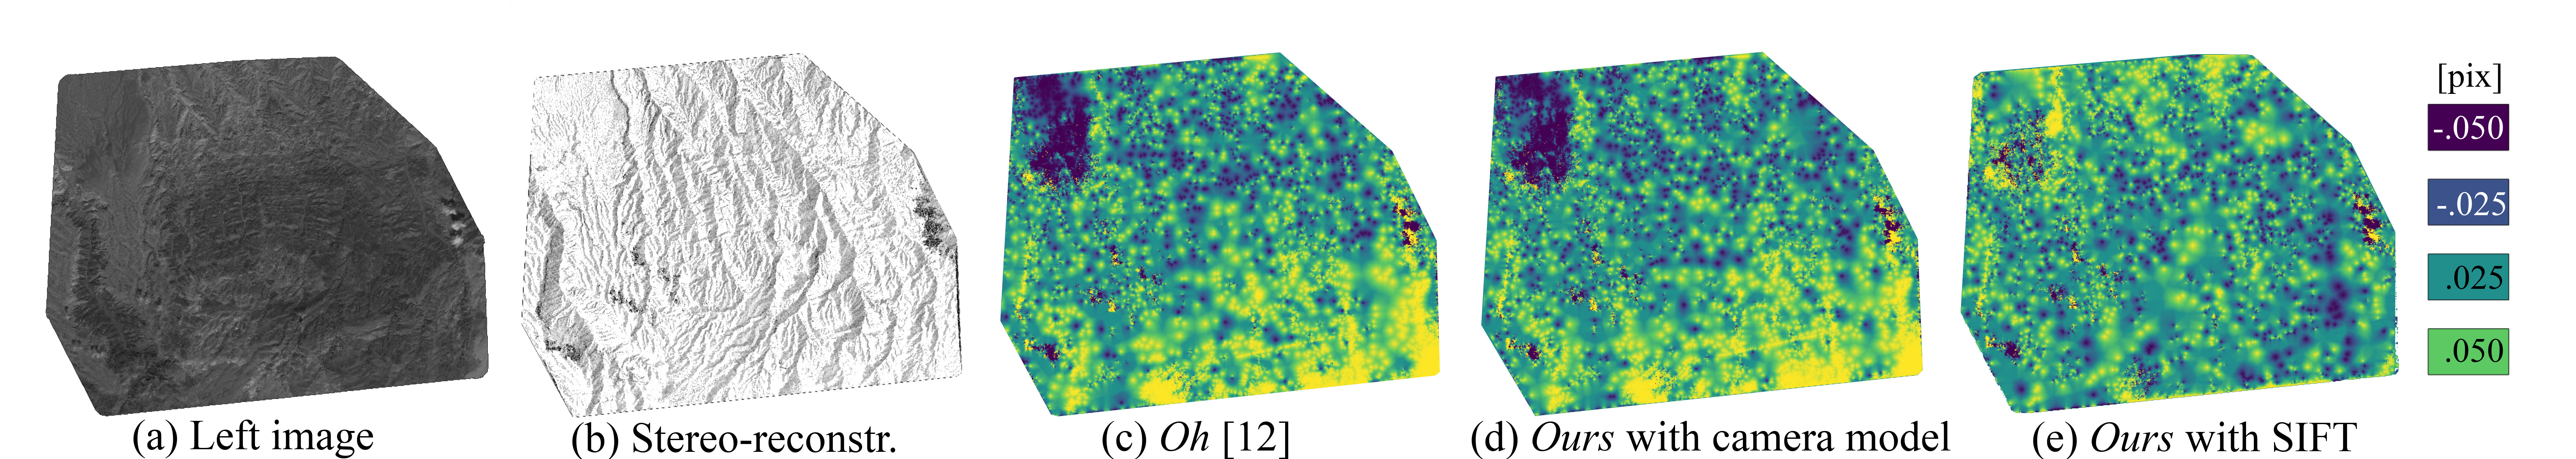
\includegraphics[width=\textwidth]{FIGS/chilli_epi_px1_px2_cmp.jpg}\caption{Comparison of epipolar resampling with and without the camera geometry. (c)-(d) correspond to the per-pixel y-parallax computed with dense image matching in the direction perpendicular to the epipolar line.}\label{fig:modelNomodelCmp}
\end{figure}
%\subsection{Radar images}

 

%\subsection{Use with pinhole camera}
%Permet de faire des test supplémentaire.

\begin{figure}%[h!]
\centering
\begin{tabular}{c}
% \hline \hline
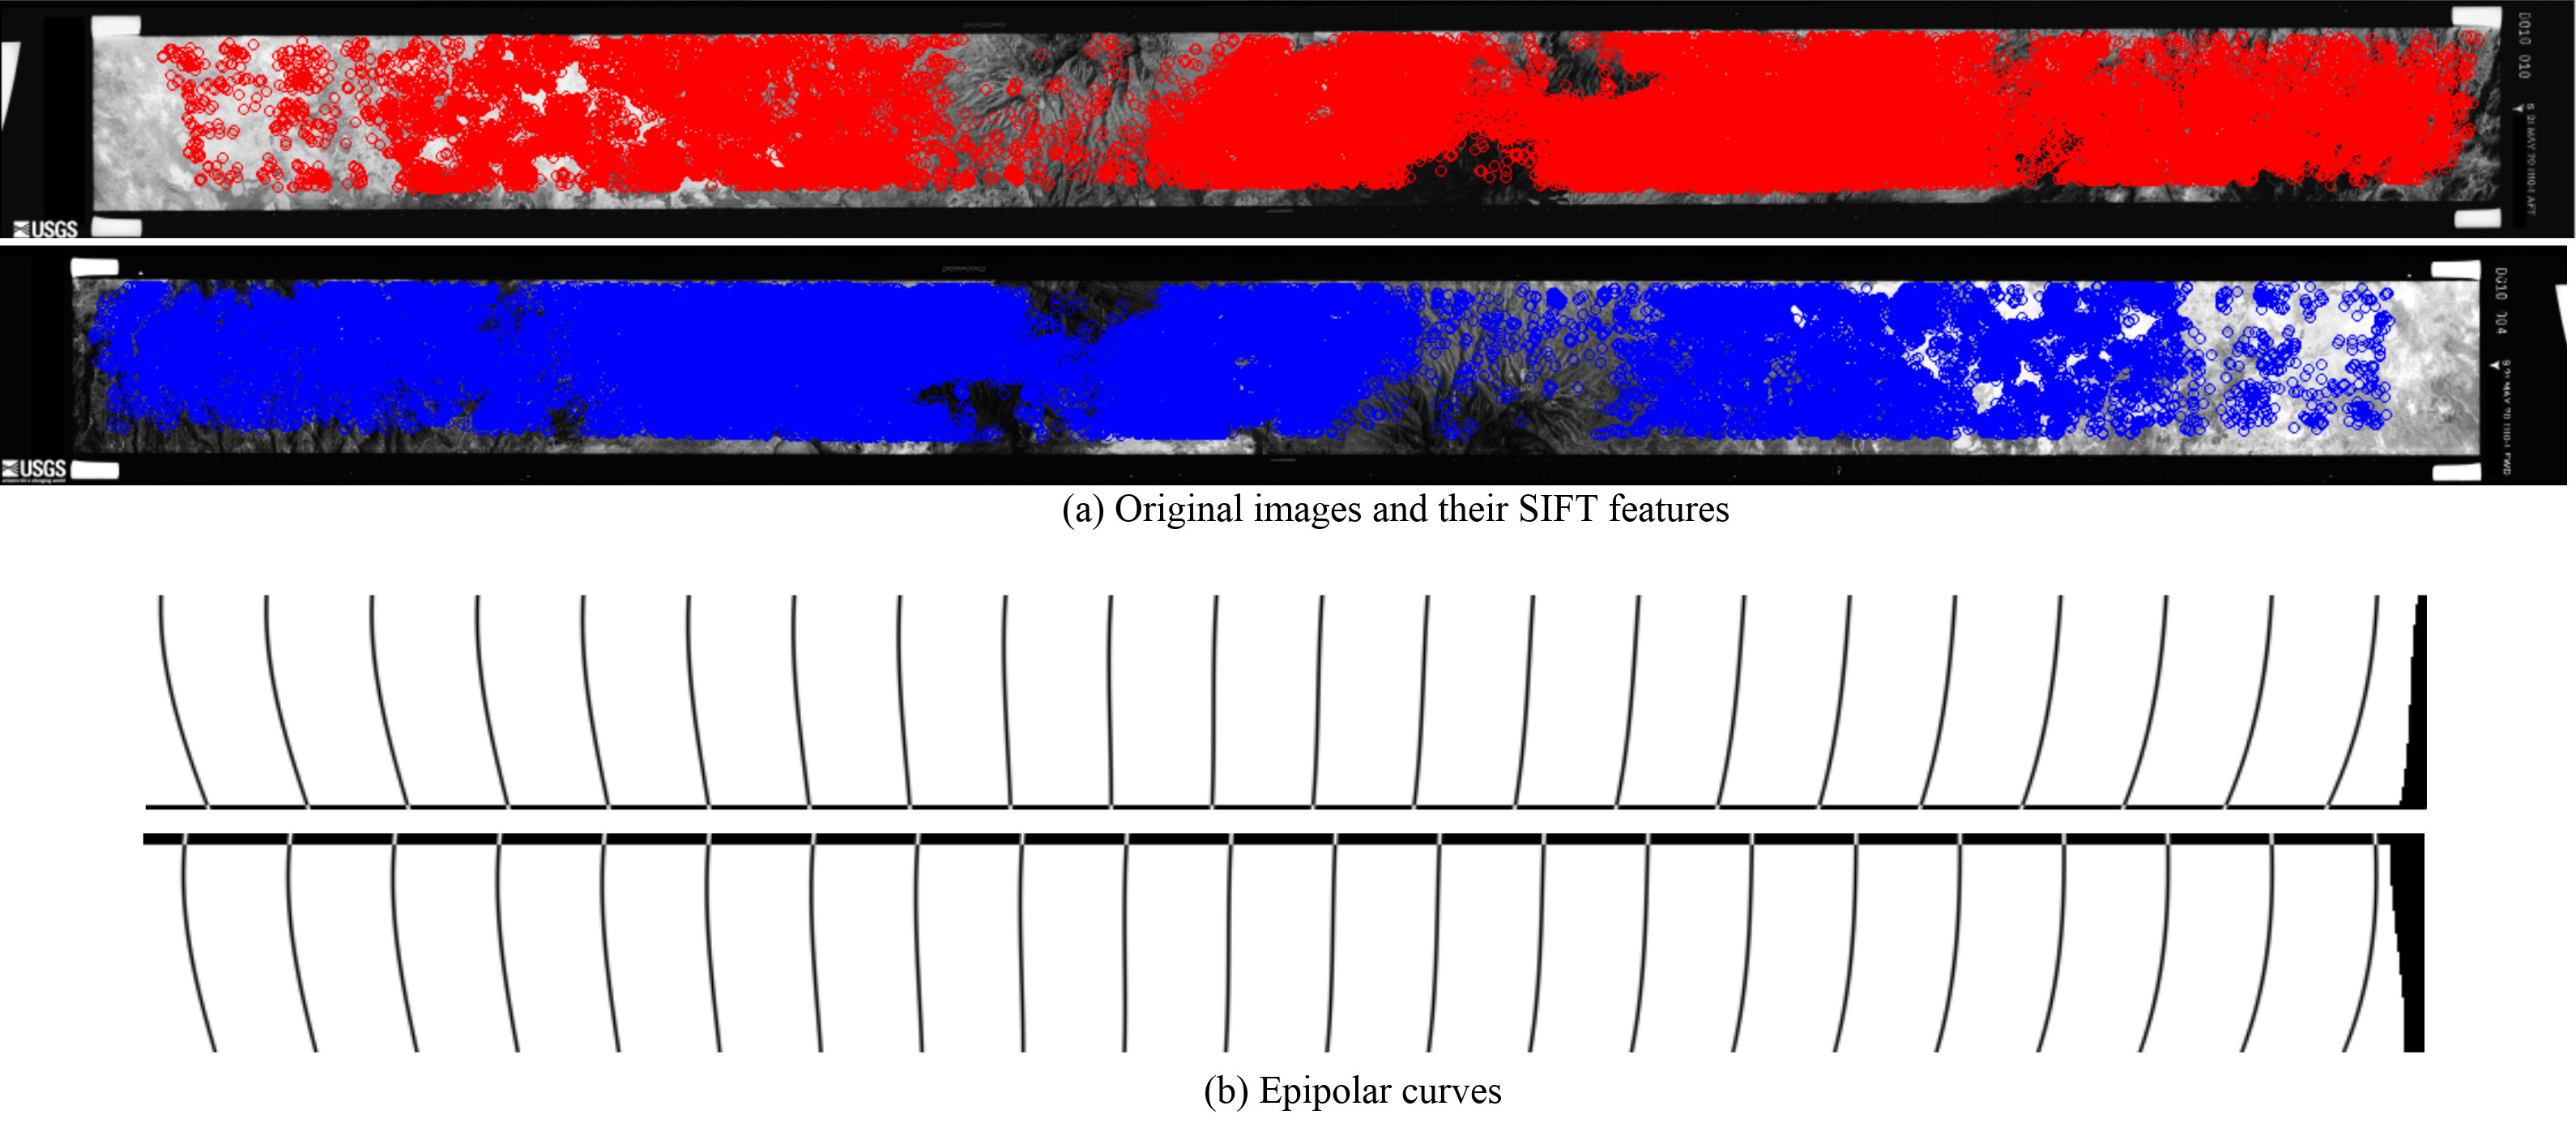
\includegraphics[width=0.9\textwidth]{FIGS/corona__sift_curves.jpg}
% \\ \hline \hline
\end{tabular}
\caption{Corona KH-4B stereo pair.}
\label{ExpCoronaSIFT}
\end{figure}
%
\begin{figure}%[h!]
\centering
\begin{tabular}{c}
% \hline \hline
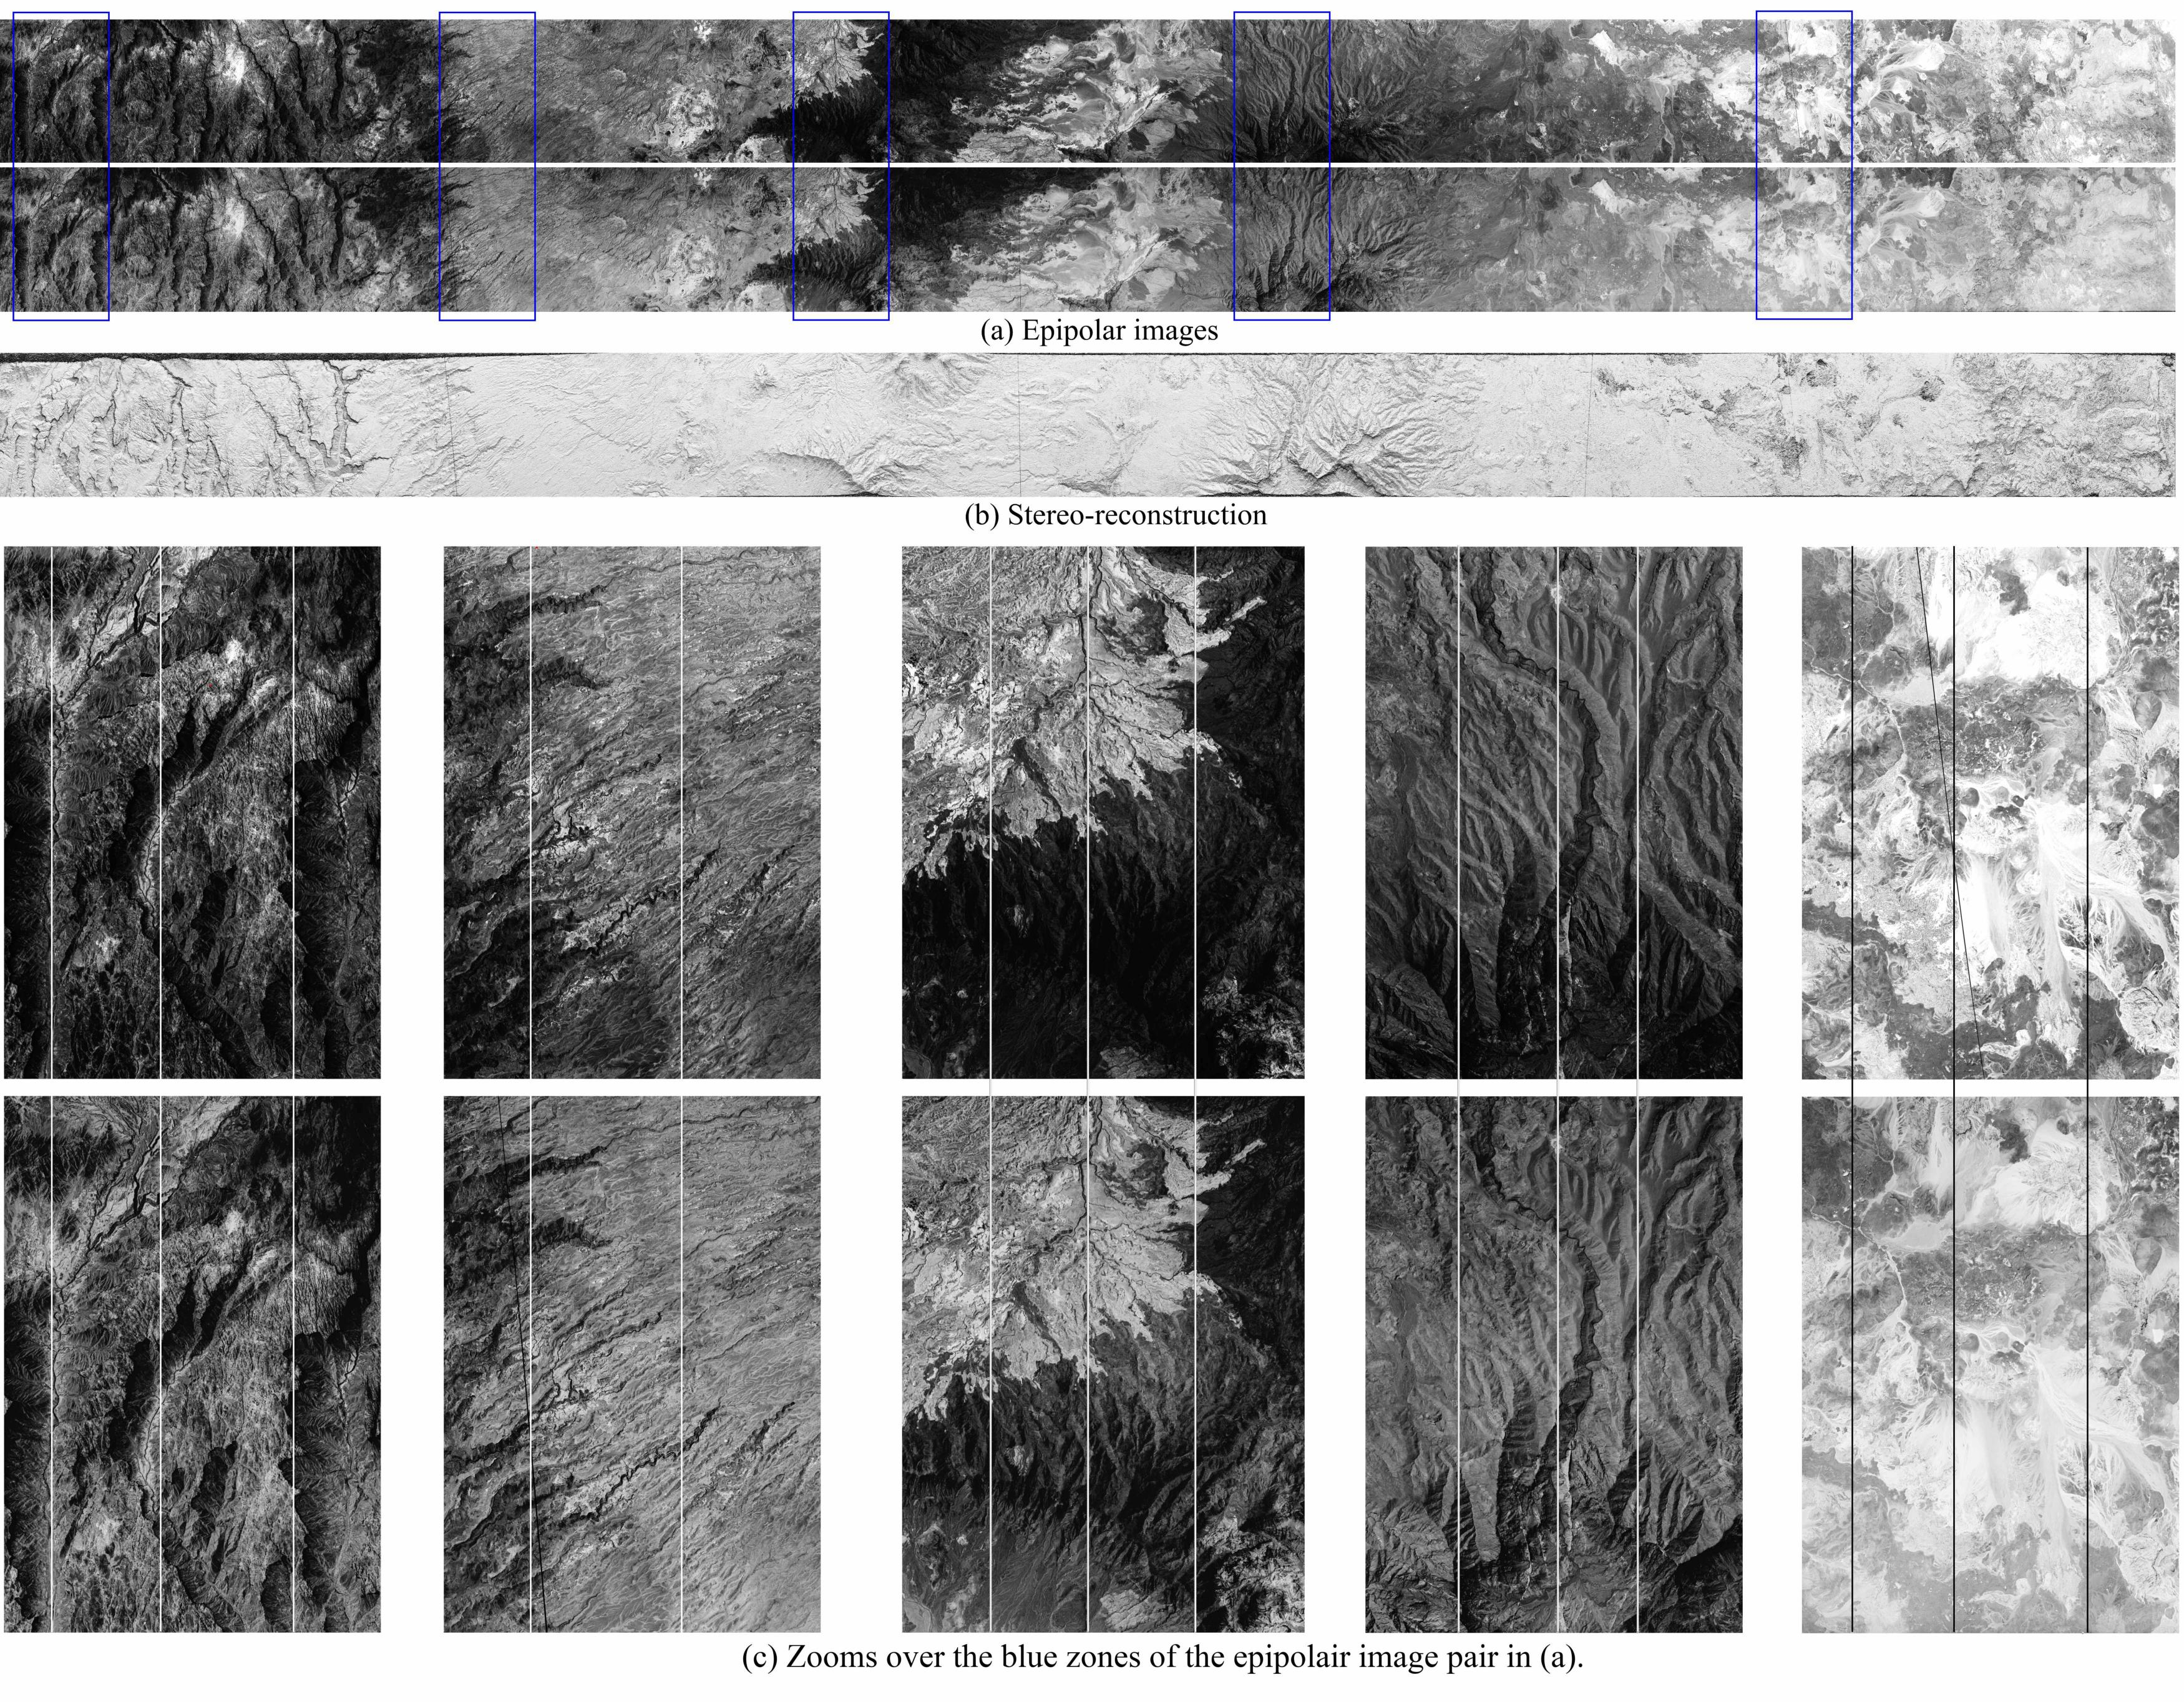
\includegraphics[width=\textwidth]{FIGS/Corona_epi_all.jpg}
% \\ \hline \hline
\end{tabular}
\caption{Epipolar images generated from a Corona KH-4B stereo pair, its stereo-reconstruction and the remaining y-parallax. Epipolar lines are marked in white.}
 
\label{ExpCoronaEpi}
\end{figure}



    
    
%\paragraph{Pl\'eiades images}
%---------------------------------------------
%---------------------------------------------


%---------------------------------------------
\begin{figure}%[h!]
\centering
\begin{tabular}{c}
% \hline \hline
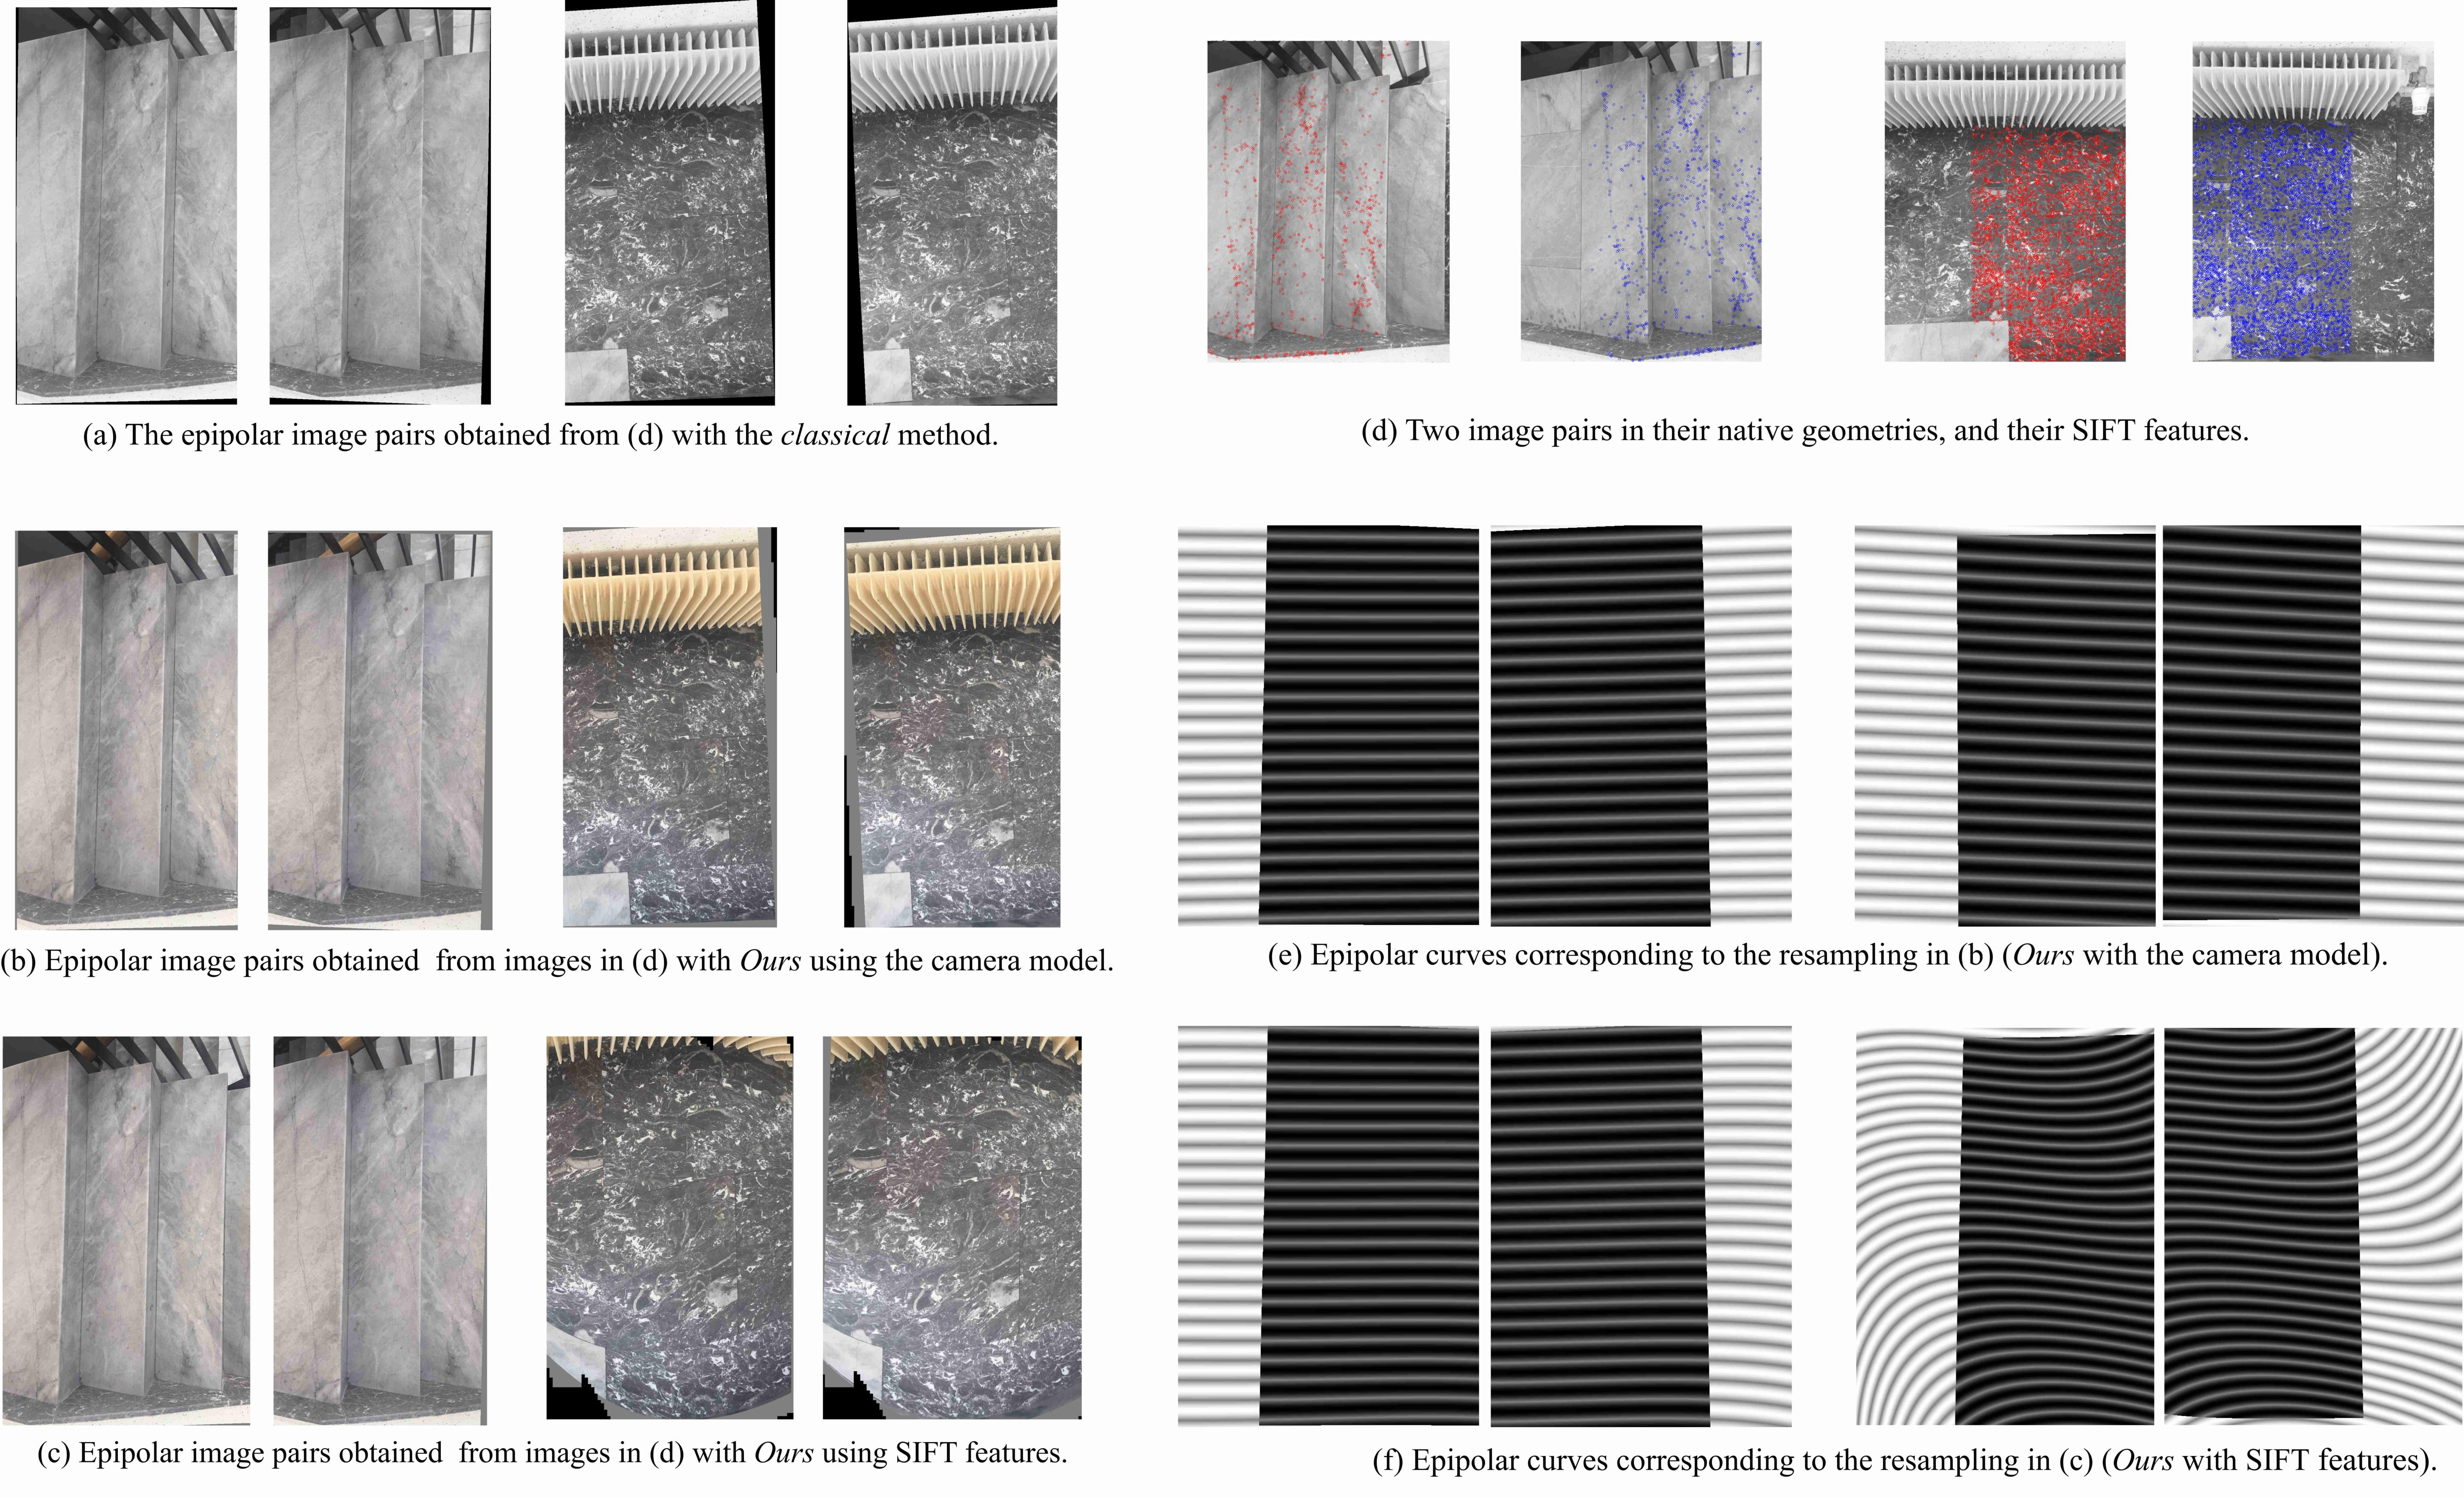
\includegraphics[width=\textwidth]{FIGS/floor_stairs_epi.jpg}
% \\ \hline \hline
\end{tabular}
\caption{Two experiments (\textit{Staircase} and \textit{Floor}) with the consumer grade camera. Epipolar pairs are obtained with three methods: the \textit{classical} being equivalent of the resampling proposed by Fusiello~\cite{fusiello2000epi} for calibrated cameras, \textit{Ours} with the camera model, and \textit{Ours} with the SIFT features. In (e) and (f) the black background corresponds to the overlapping zones in the image pairs.}
 
\label{ExpConsumerCam}
\end{figure}

 

%---------------------------------------------
%---------------------------------------------
%---------------------------------------------

\bibliographystyle{siam}
\bibliography{epip}
%\begin{thebibliography}{References}

%   \bibitem[Oh,     Jaehong. 2011]{Oh2011}
%            Oh,     Jaehong. 2011,     Novel     Approach     to     Epipolar Resampling  of  
%            HRSI  and  Satellite  Stereo  Imagery-based Georeferencing   of   Aerial   Images.Diss.
%            The   Ohio   State University.
%
%   \bibitem[De Franchis,Carlo 2015]{Franchis2015}   Earth Observation and Stereo Vision.
%           Ph Dissertation, Paris-Saclay 2015.
%
%    \bibitem[Weierstrass,Karl 1885 ]{Weierstrass1885} Über die analytische Darstellbarkeit sogenannter willkürlicher Functionen 
%           einer reellen Veränderlichen. Sitzungsberichte der Königlich Preußischen Akademie der Wissenschaften zu Berlin, 
%           1885 (II).  Erste Mitteilung (part 1) pp. 633–639, Zweite Mitteilung (part 2) pp. 789–805.
%
%    \bibitem[Stone, M. H. 1937]{Stone1937} "Applications of the Theory of Boolean Rings to General Topology", 
%          Transactions of the American Mathematical Society, Transactions of the American Mathematical Society, 
%          Vol. 41, No. 3, 41 (3): 375–481
%\end{thebibliography}

\end{document}
%-------------------------------------------------------------------------------
